%---------------------------------------------------------------------------%
%-                                                                         -%
%-                           LaTeX Template                                -%
%-                                                                         -%
%---------------------------------------------------------------------------%
%- Copyright (C) Huangrui Mo <huangrui.mo@gmail.com> 
%- This is free software: you can redistribute it and/or modify it
%- under the terms of the GNU General Public License as published by
%- the Free Software Foundation, either version 3 of the License, or
%- (at your option) any later version.
%---------------------------------------------------------------------------%
%->> Document class declaration
%---------------------------------------------------------------------------%
\documentclass[twoside,fontset=none]{Style/ucasthesis}%
%- Multiple optional arguments:
%- [<oneside|twoside|print>]% oneside eprint, twoside eprint, or paper print
%- [fontset=<adobe|none|...>]% specify font set instead of automatic detection
%- [scheme=plain]% thesis writing of international students
%- [draftversion]% show draft version information
%- [standard options for ctex book class: draft|paper size|font size|...]%
%---------------------------------------------------------------------------%
%->> Document settings
%---------------------------------------------------------------------------%
\usepackage[super,list]{Style/artratex}% document settings
%- usage: \usepackage[option1,option2,...,optionN]{artratex}
%- Multiple optional arguments:
%- [bibtex|biber]% set bibliography processor and package
%- [<numbers|super|authoryear|alpha>]% set citation and reference style
%- <numbers>: textual: Jones [1]; parenthetical: [1]
%- <super>: textual: Jones superscript [1]; parenthetical: superscript [1]
%- <authoryear>: textual: Jones (1995); parenthetical: (Jones, 1995)
%- <alpha>: textual: not available; parenthetical: [Jon95]
%- [geometry]% reconfigure page layout via geometry package
%- [lscape]% provide landscape layout environment
%- [xhf]% disable header and footer via fancyhdr package
%- [color]% provide color support via xcolor package
%- [background]% enable page background
%- [tikz]% provide complex diagrams via tikz package
%- [table]% provide complex tables via ctable package
%- [list]% provide enhanced list environments for algorithm and coding
%- [math]% enable some extra math packages
%- [xlink]% disable link colors
\usepackage{Style/artracom}% user defined commands
%---------------------------------------------------------------------------%
%->> Document inclusion
%---------------------------------------------------------------------------%
%\includeonly{Tex/Chap_1,...,Tex/Chap_N}% selected files compilation
%---------------------------------------------------------------------------%
%->> Document content
%---------------------------------------------------------------------------%
%-
%-> Titlepage information
%-
%---------------------------------------------------------------------------%
%->> Titlepage information
%---------------------------------------------------------------------------%
%-
%-> 中文封面信息
%-
\confidential{}% 密级:只有涉密论文才填写
\schoollogo[scale=0.095]{ucas_logo}% 校徽
\title{基于生成对抗网络的分类模型研究}% 论文中文题目
\author{胡兵兵}% 论文作者
\advisor{吴幼龙~助理教授~上海科技大学\\}% 指导教师:姓名 专业技术职务 工作单位
%\advisor{指导教师一\\指导教师二\\指导教师三}% 多行指导教师示例
\degree{硕士}% 学位:学士、硕士、博士
\degreetype{工学}% 学位类别:理学、工学、工程、医学等
\major{通信与信息系统}% 二级学科专业名称
\institute{中国科学院上海微系统与信息技术研究所}% 院系名称
%\institute{中国科学院力学研究所\\流固耦合实验室}% 多行院系名称示例
\date{2020~年~6~月}% 毕业日期:夏季为6月、冬季为12月
%-
%-> 英文封面信息
%-
\TITLE{Classification Models Based on Generative Adversarial Networks}% 论文英文题目
\AUTHOR{Hu Bingbing}% 论文作者
\ADVISOR{Supervisor: Professor Wu Youlong}% 指导教师
\DEGREE{Master}% 学位:Bachelor, Master, Doctor, Postdoctor。封面据英文学位名称自动切换,需确保拼写准确
\DEGREETYPE{Engineering}% 学位类别:Philosophy, Natural Science, Engineering, Economics, Agriculture 等
\MAJOR{Communication and Information System}% 二级学科专业名称
\INSTITUTE{Shanghai Institute of Microsystem and Information Technology,
Chinese Academy of Sciences}% 院系名称
\DATE{June, 2020}% 毕业日期:夏季为June、冬季为December
%---------------------------------------------------------------------------%
%
\begin{document}
%-
%-> Frontmatter: title page, abstract, content list, symbol list, preface
%-
\frontmatter% initialize the environment
%---------------------------------------------------------------------------%
%->> Frontmatter
%---------------------------------------------------------------------------%
%-
%-> 生成封面
%-
\maketitle% 生成中文封面
\MAKETITLE% 生成英文封面
%-
%-> 作者声明
%-
\makedeclaration% 生成声明页
%-
%-> 中文摘要
%-
\intobmk\chapter*{摘\quad 要}% 显示在书签但不显示在目录
\setcounter{page}{1}% 开始页码
\pagenumbering{Roman}% 页码符号

随着科技的发展,数据量日益增长,人们希望从这些原始数据中挖掘出感兴趣的信息。从一方面来看,这些数据数量庞大,所以靠人工去标注成本太高;另一方面这些高维数据复杂度高,所以常规的数据预处理方法也会失效。近年来深度学习领域研究活跃,其中生成对抗网络因其新颖的训练方式和超强的可扩展性受到了广泛关注。

本文研究了基于生成对抗网络的分类模型。传统的分类方法需要有标注的数据,而且容易过拟合,面对大量高维数据,这些方法不再适用。生成对抗网络可以无监督地进行训练,而且在模型稳定之后,生成的新数据可以用来扩充数据集。本文提出了两种基于生成对抗网络的分类模型:C-InfoGAN和InfoCatGAN。前者将InfoGAN扩展为分类模型,利用模型中的辅助网络做分类,能够在生成高质量图片的同时,达到较好的分类准确率;后者在 CatGAN 的基础上增加了互信息约束,使得生成的图片更加逼真。二者均能通过隐变量控制生成图片的类别,这对数据增强具有较大意义。此外,在加入少量标签信息之后,模型的准确率能大幅提高。

\keywords{生成对抗网络,分类,无监督学习,半监督学习}% 中文关键词
%-
%-> 英文摘要
%-
\intobmk\chapter*{Abstract}% 显示在书签但不显示在目录

As the science and technology grow, the amount of data is increasing day by day. People want to mine valuable information from these raw data. On the one hand, the amount of these data is too large, so manual labeling is unrealistic; on the other hand, these high-dimensional data have high complexity, so classic data preprocessing methods will also fail. In recent years, the deep learning community is very active, and generative adversarial network has received extensive attention for its novel training methods and super-scalability.

This thesis studies the classification models based on generative adversarial networks. Traditional classification methods require labeled data and are easy to overfit. Facing a large number of high-dimensional data, these methods are no longer applicable. Generative adversarial networks can be trained in an unsupervised manner, and the generated data from the trained model can be used to expand the data set. This thesis proposes two classification models based on generative adversarial networks: C-InfoGAN and InfoCatGAN. The former extends InfoGAN into a classification model, and uses the auxiliary network in the model for classification, which can achieve high classification accuracy while generating high-quality pictures; the latter adds mutual information constraints to CatGAN, making the generated pictures more realistic. Additionally, both two models can control the category of generated pictures through latent variables, which has great significance for data augmentation. In addition, after adding a small amount of label information, the accuracy of the model can be greatly improved.

\KEYWORDS{GAN, Classification, Unsupervised Learning, Semi-supervised Learning}% 英文关键词
%---------------------------------------------------------------------------%
% title page, abstract
{% content list region
\linespread{1.2}% local line space
\intobmk*{\cleardoublepage}{\contentsname}% add link to bookmark
\tableofcontents% content catalog
\intobmk*{\cleardoublepage}{\listfigurename}% add link to bookmark
\listoffigures% figure catalog
\intobmk*{\cleardoublepage}{\listtablename}% add link to bookmark
\listoftables% table catalog
}
\intobmk\chapter*{符号列表}% 显示在书签但不显示在目录

\section*{字符}
\nomenclatureitem[\textbf{Unit}]{\textbf{Symbol}}{\textbf{Description}}
\nomenclatureitem[$\Unit{m^{2} \cdot s^{-2} \cdot K^{-1}}$]{$R$}{the gas constant}
\nomenclatureitem[$\Unit{m^{2} \cdot s^{-2}}$]{$E$}{specific total energy}
\nomenclatureitem[$\Unit{kg \cdot m^{-1} \cdot s^{-2}}$]{$\tau_{ij}$}{viscous stress tensor}
\nomenclatureitem[$\Unit{1}$]{$I_{ij}$}{identity tensor}
\nomenclatureitem{DUnif(a,b)}{区间[a,b]上的离散均匀分布}
\nomenclatureitem{Unif(a,b)}{区间[a,b]上的连续均匀分布}
\nomenclatureitem{$p$}{概率分布}
\nomenclatureitem{$\Pr$}{事件概率,概率测度}
\nomenclatureitem{$\mathbf{x}$}{数学加粗表示矢量}

\section*{算子}
\nomenclatureitem{\textbf{Symbol}}{\textbf{Description}}
\nomenclatureitem{$\Delta$}{difference}
\nomenclatureitem{$\nabla$}{gradient operator}

\section*{缩写}
\nomenclatureitem{CFD}{Computational Fluid Dynamics}

% symbol list, preface content
%-
%-> Mainmatter
%-
\mainmatter% initialize the environment
%---------------------------------------------------------------------------%
%->> Main content
%---------------------------------------------------------------------------%
%\input{Tex/Chap_Intro}
\chapter{绪论}\label{chap:introduction}

\section{研究背景}
\section{研究现状}
\section{本文贡献}
\section{本文结构}
%\chapter{预备知识}\label{chap:preliminaries}
\section{引言}
在开始介绍本文工作之前,首先需要了解一些背景知识。本章首先介绍什么是生成式模型和判别式模型,然后给出生成对抗网络的详细介绍及其数学模型,最后介绍InfoGAN和CatGAN模型。

\section{生成式模型和判别式模型}\label{sec:gm-dm}
在介绍生成对抗网络之前,我们有必要了解两个概念:生成式模型(Generative Modeling, GM)和判别式模型(Discriminative Modeling,DM)。我们先用简单地一句话说明,接着再详细阐述它们区别。简而言之,生成式模型研究的是数据和标签之间的联合分布,而判别式模型研究的是标签关于数据的条件分布。

在一个基本的机器学习问题中,通常有输入$x \in \Set{X}$和输出$y \in \Set{Y}$两个部分。通俗的说,DM关注$x$和$y$的内在联系,即在给定$x$的条件下,$y$的分布应该满足什么样的性质;
而GM更关注于$(x, y)$的联合分布。模型训练完成之后,判别式模型将训练数据集的信息提取,模型本身拟合了训练样本中的经验条件分布$P(y|x)$,因此对于测试样本$x^{\star}$,判别式模型直接输出对应的条件概率$P(y^{\star} | x^{\star})$,给出分类结果。生成式模型则对训练集的联合分布$P(x,y)$进行建模,对于未见样本$x^{\star}$,选择使得$P(x^{\star}, y)$最大的$y$作为预测值。由贝叶斯公式知
\[
  \begin{split}
    y^{{\star}} &= \argmax_y P(y|x^{{\star}}) \\
       &= \argmax_y \frac{P(x^{\star}|y)P(y)}{P(x^{\star})} \\
       &= \argmax_y P(x^{\star}|y)P(y) \\
       &= \argmax_y P(x^{\star}, y).
  \end{split}
\]
因此,这等价于寻找使得$P(y|x^{\star})$最大的$y$作为预测值。

常见的生成式模型有:朴素贝叶斯(Naive Bayes)、高斯混合模型(Gaussian Mixture Model,GMM)、受限玻尔兹曼机(Restricted Boltzmann Machine,RBM);常见的判别式模型有:KNN(K-Nearest Neighbours)、逻辑回归(Logistic Regression)、感知机(Perceptrons)、决策树(Decision Tree)、条件随机场(Conditional Random Field)等。
在实际使用中,两者各有优劣。生成式模型可以建模联合分布,但联合分布本身难以估计,所以会需要较大地数据量和计算量。判别式模型具有更低地渐近误差,但其收敛到渐近误差的速度比生成式模型更慢;而生成时模型的渐近误差往往高于判别式模型\citep{ng2002discriminative},而且可以处理隐变量和半监督甚至无监督学习。


%一般来说,判别式模型比生成式模型更受欢迎,特别是在分类问题中,判别式模型直接建模$P(y|x)$进行分类,而生成式模型则先建模$P(x,y)$然后再计算$P(y|x)$进行分类。首先联合概率的估计本身比较困难,因此需要耗费更多的数据量和计算资源。


\section{生成对抗网络}
\subsection{基本思想}
\citet{goodfellow2014generative}在2014年提出生成对抗网络,该模型使用博弈理论中的minimax博弈机制来训练两个模块:生成器和判别器。
%其目标是学习一个生成器对应的分布$p_g$使得它和真实数据的分布$p_{\text{data}}$尽量接近。
其目标时通过交替更新生成器和判别器,通过二者的对抗使得生成器学习到真实的数据分布,即令生成器对应的分布$p_g$和真实数据的分布$p_{\text{data}}$尽量接近。
生成式模型不直接估计每个数据样本的概率,而是利用生成网络$G$将噪声变量$\bd{z} \sim p_z(\bd{z})$映射到虚假样本$G(\bd{z})$。在训练过程中,判别器的目标是将虚假样本和真实样本区分开,生成器的目标则是生成让判别器无法区分的虚假样本。训练过程可以类比为两个玩家博弈:判别器读取一个数据希望能够分判定其是否为真实样本,而生成器希望生成以假乱真的数据从而让判别器判定为真。整个过程大致如下:生成器将一个随机噪声映射到数据空间,形成一个虚假数据。判别器接受真实样本或虚假样本作为输入,并输出当前样本来自真实数据的概率。训练的目标是一方面让判别器能够区分真假,一方面使生成器能够以假乱真,这就形成了两方对抗,最终二者的能力越来越强,无法进一步提高自己的性能,博弈达到平衡点。
\begin{figure}[htbp]
  \centering
  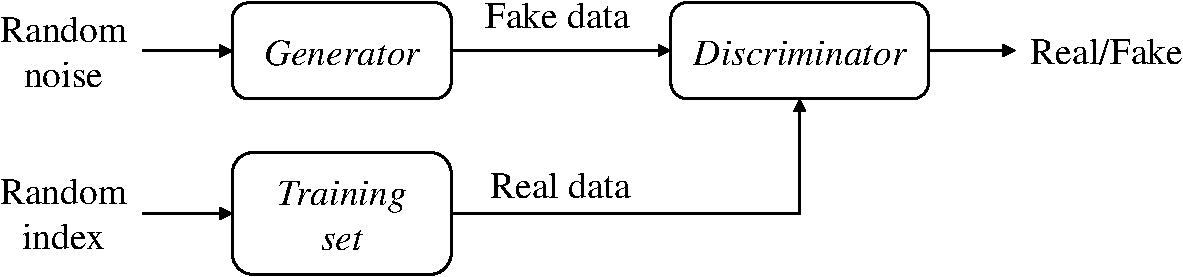
\includegraphics[width=0.9\textwidth]{Img/arch-gan.pdf}
  \bicaption{朴素GAN结构示意}{The architecture of vanilla GAN}
  \label{fig:arch-gan}
\end{figure}

\subsection{数学模型}
设$\Set{X} = \{\bd{x}_1, \cdots, \bd{x}_N\}$为含有$N$个样本的数据集,$\bd{x}_i = (x_{i1}, \cdots, x_{in}) \in \reals^n$为单个数据样本,标准生成对抗网络模型可被正式定义如下:生成器$G: \reals^m \mapsto \reals^n$,判别器$D: \reals^n \mapsto [0, ~1]$。其中$m$为隐空间维度,即噪声维度,$n$为数据维度。给定输入噪声$\bd{z} \sim p_z, \bd{z} = (z_1, \cdots, z_m) \in \reals^m$,$G(\bd{z}) \in \reals^n$为生成器生成的虚假样本;给定真实数据样本$\bd{x}$或虚假样本$G(\bd{z})$,$D(\cdot) \in [0,~1]$表示当前输入来自真实数据的概率。接着训练$D$使得对于真实数据$\bd{x}$,$D(\bd{x})$接近于$1$;对于虚假数据$\tilde{\bd{x}} = G(\bd{z})$,$D(\tilde{\bd{x}})$接近于$0$。同时训练$G$使得$\log(1 - D(G(\bd{z}))$达到最小。换言之,$D$和$G$类似两个玩家博弈,其价值函数如下:
\begin{equation}
  \min_G\max_D ~V(D,G) =
    \E_{\bd{x} \sim p_{\text{data}}}[\log D(\bd{x})] + 
    \E_{\bd{z} \sim p_z}[\log(1-D(G(\bd{z})))].
  \label{eq:gan-obj}
\end{equation}

在实际应用中,GAN通常被实现为可微神经网络:生成器网络$G(\cdot; {\theta}_g)$和判别器网络$D(\cdot; {\theta}_d)$,其中${\theta}_g$和${\theta}_d$分别为生成器和判别器的网络参数\footnote{为了简便起见,在不产生歧义的情况下通常省略网络参数。}。此外,生成器和判别器在实现中也需要采用交替迭代的机制,使用基于梯度的优化方法来训练。在训练初期,$G$生成的加虚假样本比较容易被$D$识别,从\eqref{eq:gan-obj}式可以看出,$\log(1 - D(G(\bd{z})))$的梯度变化很小,生成器难以得到优化。因此,在实现中通常训练$G$使得$\log D(G(\bd{z}))$达到最大。

%----------------------------------------------------------------------
\section{InfoGAN}\label{sec:infogan}
\subsection{基本思想}
朴素GAN通常使用高维高斯噪声作为生成器的输入,并没有规定生成器如何利用这个噪声,也没有对隐空间作任何限制。因此,噪声的利用可以是任意的,生成器可能生成具有高度耦合特征的数据。这从图像上来看,也就是模型生成的虚假图片高度抽象,没有明显轮廓。从底层来看,$\bd{z}$的每一维度并没有对应到生成数据的某个特征。然而,一个好的模型很自然地可以将数据的各个特征分离出来,以提供给用户调整。比如,当要求GAN从MNIST\citep{lecun1989backpropagation}生成图片时,理想的模型可以利用一个离散随机变量来表示数字类别特征(0-9),利用两个连续随机变量来分别表示数字的角度和笔画的粗细。

\citet{mirza2014conditional,odena2017conditional,miyato2018cgans}均指出通过调整隐空间结构,可以控制生成器生成具有某个特征的图片。InfoGAN\citep{chen2016infogan}将隐变量分解为两部分,一部分仍然是无结构的噪声$\bd{z} \sim p_z$,为模型提供足够的容量;另一部分则作为隐变量$\bd{c} \sim p_c$,用于学习数据特征。

\subsection{互信息约束}
设$\bd{c} = (c_1, c_2, \cdots, c_t)$表示输入空间中的$t$个隐变量,最简单的情况是各隐变量之间互相独立,即$p_{\bd{c}}(c_1, c_2, \cdots, c_t) = \prod_{i=1}^t p_{c_i}(c_i)$。InfoGAN基于朴素GAN模型提出了一种在无监督条件下,利用隐变量学习到数据特征的方法。该方法将隐空间噪声分解为两部分,包含一个生成器$G(\bd{z}, \bd{c})$和一个判别器$D$。由于在朴素GAN中,生成器可以忽略隐空间结构,此时$p_g(x|c) = p_g(x)$,其中$p_g$为生成器对应的概率分布。为了解决这个问题,InfoGAN为模型增加了互信息正则项,并指出隐变量$\bd{c}$和生成数据$G(\bd{z}, \bd{c})$之间的互信息应该很高。
\begin{figure}[hbtp]
  \centering
  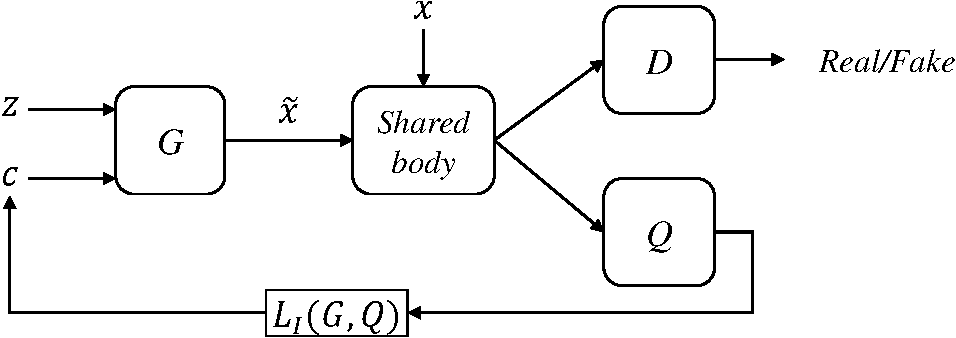
\includegraphics[width=0.75\textwidth]{Img/arch-infogan.pdf}
  \bicaption[InfoGAN结构示意]{InfoGAN结构示意。其中$\bd{x}$表示真实样本,$\tilde{\bd{x}} = G(\bd{z},\bd{c})$表示由生成器生成的虚假样本。在实现中,通常将辅助网络$Q$和判别器$D$共享一部分网络结构。}{The architecture of InfoGAN. $\bd{x}$ denotes the real data and $\tilde{\bd{x}} = G(\bd{z}, \bd{c})$ denotes fake data. In practice, $Q$ and $D$ share a body.}
  \label{fig:arch-infogan}
\end{figure}

在信息论中,熵(Entropy)、相对熵(Relative Entropy)以及互信息(Mutual Information)的定义如下\citep{cover2012elements}:
\begin{definition}{熵}
  设有离散随机变量$X \sim p_X(x)$及其支撑集$\Set{X}$,则它的熵$H(X)$定义为
  \begin{equation}
    H(X) = -\sum_{x\in\Set{X}} p_X(x) \log p_X(x).
  \end{equation}
  \label{def:entropy}
\end{definition}
\begin{definition}{KL距离}
  设有定义在同一个支撑集$\Set{X}$上的两个概率分布$p(x)$和$q(x)$,则它们的相对熵(或称Kullback-Leibler距离)定义为
  \begin{equation}
    D_{\text{KL}}(p~||~q) = \sum_{x\in\Set{X}} p(x)\log \frac{p(x)}{q(x)}.
  \end{equation}
  \label{def:relative-entropy}
\end{definition}
\begin{definition}{互信息}
  设$X,~Y$是两个离散随机变量,它们的支撑集分别为$\Set{X},~\Set{Y}$,它们的联合分布为$p_{X,Y}(x, y)$,边缘分布分别为$p_X(x)$和$p_Y(y)$,则$X$和$Y$之间的互信息$I(X;~Y)$定义为它们联合分布和边缘分布乘积之间的相对熵:
  \begin{equation}
    \begin{split}
      I(X;~Y) &= \sum_{x\in\Set{X}}\sum_{y\in\Set{Y}} 
      p_{X,Y}(x,y) \log\frac{p_{X,Y}(x,y)}{p_X(x) \cdot p_Y(y)}  \\
            &= D_{\text{KL}}\left( p_{X,Y}(x,y)~||~p_X(x) p_Y(y) \right) \\
            &= \E_{p_{X,Y}} \left[ 
              \log\frac{p_{X,Y}}{p_X \cdot p_Y}
              \right].
    \end{split}
    \label{eq:mutual-information}
  \end{equation}
  \label{def:mutual-information}
\end{definition}

在信息论中,熵度量着随机变量的其不确定性,用来衡量它所持有的信息量。由以上定义,容易得到
\begin{equation}
  \begin{split}
    I(X;~Y) &= H(X) - H(X|Y) \\
    &= H(Y) - H(Y|X).
  \end{split}
\end{equation}
可知随机变量$X,~Y$的互信息度量着观测到$Y$之后,$X$的不确定性的减少量。从\eqref{eq:mutual-information}式可以看出,互信息越大表明两个随机变量之间的相关性越大,反之互信息为零则说明变量间相互独立。于是,最大化隐变量$\bd{c}$和生成器输出$\tilde{\bd{x}} = G(\bd{z}, \bd{c})$的互信息$I(\bd{c}; ~\tilde{\bd{x}}) = H(\bd{c}) - H(\bd{c}|\tilde{\bd{x}})$等价于最小化$H(\bd{c}|\tilde{\bd{x}})$,这里由于$\bd{c}$的分布在整个过程中是确定的,所以$H(\bd{c})$可以视为常数。换句话说,隐变量$\bd{c}$的信息量在生成过程中应该流向$\tilde{\bd{x}}$,即给定$\tilde{\bd{x}}$之后,$\bd{c}$的信息量应该很小。类似的互信息约束也可以应用到聚类中\citep{bridle1992unsupervised,barber2006kernelized,krause2010discriminative}。InfoGAN在朴素GAN的基础上增加了互信息约束,其价值函数$V_I(D,G)$如下:
\begin{equation}
  \min_G\max_D ~V_I(D,G) = V(D,G) - \lambda I(\bd{c};~G(\bd{z},\bd{c})).
\end{equation}


\subsection{互信息的变分下界及其估计}
在实际应用中,由于依赖后验信息$p_{\bd{c}|\tilde{\bd{x}}}(c|x)$,互信息$I(\bd{c};~G(\bd{z},\bd{c}))$难以直接计算。\citet{poole2019variational}提出互信息的变分下界
\begin{equation}
  \begin{split}
    I(\bd{c}; \tilde{\bd{x}}) 
    &= \E_{ p_{\bd{c},\tilde{\bd{x}}} } \left[ 
      \log \frac{ p_{\bd{c},\tilde{\bd{x}}}(c, x) } 
                { p_{\bd{c}}(c) p_{g}(x) }
              \right] 
      = \E_{ p_{\bd{c},\tilde{\bd{x}}} } \left[ 
      \log \frac{ p_{\bd{c}|\tilde{\bd{x}}}(c|x) }
                { p_{\bd{c}}(c) }
              \right] \\
      &= \E_{ p_{\bd{c}, \tilde{\bd{x}}} } \left[
      \log \frac{ Q(c|x) }
                { p_{\bd{c}}(c) } 
              \right]
    + \E_{p_g(x)} \left[ 
      D_{\text{KL}} \left( p_{\bd{c}|\tilde{\bd{x}}}(c|x) ~||~ Q(c|x)
                    \right)
                  \right] \\
    &\ge \E_{ p_{\bd{c},\tilde{\bd{x}}} } \left[
      \log Q(c|x) \right] + H(\bd{c}) 
      \triangleq L_I(Q(c|x)),
  \end{split}
  \label{eq:vlb}
\end{equation}
其中$p_{\bd{c}}$为隐变量分布,$p_g$为生成器对应的概率分布,$Q(c|x)$为InfoGAN模型的辅助网络用以估计真实后验概率$p_{\bd{c}|\tilde{\bd{x}}}(c|x)$,$L_I(Q(c|x))$即为互信息的变分下界。在训练过程中,隐变量的分布是固定的,所以$H(\bd{c})$可视为常量。事实上,下界$L_I$与生成器和辅助网络都有联系:
\[
  L_I(G,Q) = \E_{ p_{\bd{c},\tilde{\bd{x}}} } \left[
  \log Q(c|G(\bd{z},\bd{c})) \right] + H(\bd{c}).
\]
从\eqref{eq:vlb}式可以看出,随着辅助分布$Q$接近真实后验分布,即
\[
  \E_{p_g(x)}[D_{\text{KL}}(p_{\bd{c},\tilde{\bd{x}}}(\cdot|x) ~||~ Q(\cdot|x))] \to 0,
\]
变分下界越来越紧。综上所述,InfoGAN的目标函数如下:
\begin{equation}
  \min_{G,Q}\max_D ~V_{\text{InfoGAN}}(D,G,Q) = V(D,G) - \lambda L_I(G,Q),
  \label{eq:infogan-obj}
\end{equation}
其中$\lambda$为正则系数。




%----------------------------------------------------------------------
\section{CatGAN}\label{sec:catgan}
\ref{sec:gm-dm}节提到生成式模型适合用于半监督甚至无监督学习,CatGAN\citep{springenberg2015unsupervised}就是研究无监督和半监督分类的模型。

\subsection{基本思想}
朴素GAN模型的判别器的输出是一个概率,代表着当前输入来自真实数据的概率。如前所述,GAN的训练过程可以表述如下。设有真实数据集$\Set{X} = \{\bd{x}_1, \cdots, \bd{x}_N\}$,$\bd{x}_i \in \reals^n$, $N$为数据样本个数。生成器$G$将噪声$\bd{z}\in \reals^m$映射到数据空间,生成虚假样本$\tilde{\bd{x}} = G(\bd{z})$。判别器$D$输出样本$x$来自真实数据集$\Set{X}$的概率:$\Pr(y=1 | x) = \frac{1}{1 + e^{-D(x)}}$。\eqref{eq:gan-obj}式可以写为如下等价形式:
\begin{equation}
  \min_G\max_D ~\E_{\bd{x} \sim p_{\text{data}}} \left[ \log \Pr(y=1|\bd{x}) \right]
  + \E_{\bd{z} \sim p_z} \left[ \log\left( 1 - \Pr(y=1|G(\bd{z})) \right) \right],
\end{equation}
其中$p_{\text{data}}$和$p_z$分别表示数据分布和噪声分布。朴素GAN没有对噪声分布作任何限制,CatGAN令$p_z = \text{Unif}(0,1)$,即连续均匀分布。

基于以上陈述,CatGAN提出了一种新的生成对抗网络结构来作无监督和半监督学习。首先考虑无监督的设定,无监督条件下的结构是针对朴素GAN的推广。

\subsection{问题建模}\label{sec:catgan-ps}
如前所述,设$\Set{X} = \{\bd{x}_1, \cdots, \bd{x}_N\}$为$N$个无标注数据样本。考虑以无监督的方式,从数据$\Set{X}$学习一个判别器$D$,使得$D$将给定数据划分到事先确定好的$K$个类别之一。进一步地,我们要求$D(\bd{x})$给出$\bd{x}$属于每个类别的概率:$\sum_{k=1}^K \Pr(y=k|\bd{x}) = 1$。CatGAN的目标是训练这样一个概率分类器,使其在分配概率时满足某种要求。注意到真实的标签分布是未知的,无法直接最大化对数似然函数,所以CatGAN了设计一个鉴定分类器性能的度量方式。具体说来,如果对于给定样本$\bd{x}$,$D$输出的条件分布$p(y|\bd{x})$具有很高的确定性,而边缘分布$p(y)$对于所有$k \in \{1,2,\cdots,K\} \triangleq [K]$都接近某个先验分布$p_Y$。在整个推导过程中,CatGAN假设标签的先验分布$p_Y$为类别均匀分布,也就是说$\Set{X}$中每个类别的样本数量大致相等:$\forall k_1, ~k_2 \in [K], ~\Pr(y=k_1) = \Pr(y=k_2)$。

上述问题的建模可以自然联想到软聚类问题,所以理论上来说可以用概率聚类算法如:Regularized information maximization (RIM) \citep{krause2010discriminative},或者最小化相对熵\citep{grandvalet2005semi}。然而一旦数据集中存在一些虚假相关性,这些方法就容易生过拟合。第二个直观感觉是朴素GAN的结构无法直接用来解决这个问题,因为朴素GAN的判别器只能输出一个概率以判断真假,而不能判断输入到底来自哪个类别。原则上,我们希望一个分类器可以建模数据分布,同时学习到数据特征加以利用进行下一步操作,比如判别式聚类。然而,判别器并不一定只能区分真假(二分类),它也应该能够将输入分配到多个类别。

尽管可能存在一些问题,但是一个非常简单的做法是将朴素GAN结构扩展一下使得判别器可被用于多分类任务。一旦$D$的结构改变,那么朴素GAN模型的对抗机制则需要重新设计。CatGAN将博弈机制改变为:要求判别器将每个真实数据样本划分到$K$个类别中的一个,而对于虚假样本,保持一个较高的不确定性。这样可以让分类器更加鲁棒。类似地,要求生成器生成具体到某个类别的图片而不是仅仅生成和真实数据类似的图片。

\subsection{目标函数}
如前所述,CatGAN所定义的优化问题与朴素GAN的不同之处主要在于:CatGAN想要学习一个判别器,它能够为每个真实数据样本$\bd{x}$附加一个标签$y \in [K]$而非学习一个二分类的判别器。定义判别器$D(\bd{x})$为可微函数,它输出一个$K$维对数概率向量(logits):$D(\bd{x}) \in \reals^K$。样本$\bd{x}$属于每个类别的概率可以通过对判别器输出施加softmax变换获得:
\begin{equation}
  \Pr(y=k|\bd{x}) = \frac{e^{D_k(\bd{x})}}{\sum_{k=1}^K e^{D_k(\bd{x})}},
\end{equation}
其中$D_k(\bd{x})$表示$D(\bd{x})$的第$k$个分量。和朴素GAN一样,生成器$G(\bd{z})$定义为将噪声$\bd{z} \in \reals^m$映射到数据空间$\tilde{\bd{x}} \in \reals^n$的函数:
\begin{equation}
  \tilde{\bd{x}} = G(\bd{z}), \quad \bd{z} \sim p_z,
\end{equation}
其中$p_z$表示噪声分布。

\begin{figure}[hbtp]
  \centering
  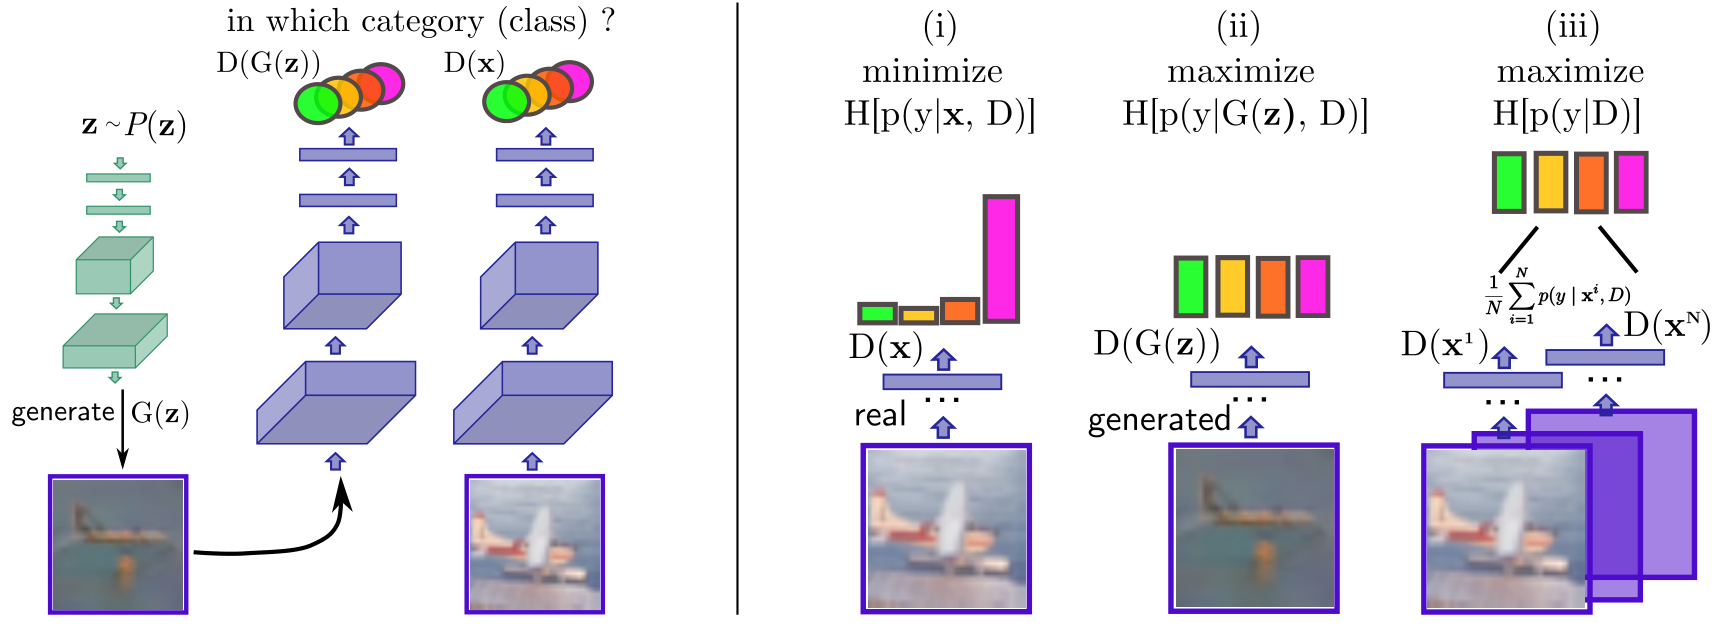
\includegraphics[width=0.9\textwidth]{Img/arch-catgan.png}
  \bicaption[CatGAN结构示意]
  {左图为CatGAN结构示意,绿色为生成器,紫色为判别器。右图为CatGAN判别器目标$L_D^{cat}$的直观解释。给定真实样本,判别器的输出呈单峰分布;给定虚假样本,判别器的输出呈均匀分布;对于所有真实图片,标签$y$的边缘分布呈均匀分布。}
  {The architecture of CatGAN is shown on the left, where generator is green and discriminator is violet. An intuitive interpretation of the objective function $L_D^{cat}$ for the discriminator is shown on right. For real samples, miminizing $H(p(y|\mathbf{x}))$ leads to single peak distribution; for fake samples, maximizing $H(p(y|G(\mathbf{z})))$ leads to uniform distribution. Finally, maximizing the marginal class entropy over all data-points leads to uniform usage of all classes.}
  \label{fig:arch-catgan}
\end{figure}

如\ref{sec:catgan-ps}节所说,如何度量分类器性能呢?CatGAN本意其实是让生成器作为判别器的正则项,使得判别器对于虚假样本更加鲁棒。基于这个想法,CatGAN提出了3条判别器需要满足的要求和2条生成器需要满足的要求:
\begin{itemize}
  \item[\textbf{判别器}](i) 对真实数据样本具有很高的确定性,(ii) 对于虚假样本具有很高的不确定性,(iii) 均匀使用所有类别\footnote{因为CatGAN假设标签的先验分布是类别均匀的。}。
  \item[\textbf{生成器}](i) 生成虚假样本使得判别器对其具有较高的确定性,(ii) 生成的样本均匀的分布在$K$个类别中。
\end{itemize}

CatGAN将这些要求都转化为可优化的条件概率,以此设计出目标函数。注意,在$K$个类别信息未知的情况下,我们无法直接优化条件概率$\Pr(y=k|\bd{x})$以满足判别器的第一个要求。因此,只能通过信息论中的一些尺度直接对分布信息进行刻画。最常用的信息论尺度就是熵。直观来看,对于真实样$\bd{x}$,我们想让条件分布$p(y|\bd{x})$呈现单峰趋势(即$D$很确定将当前样本划分到哪个类别),可以通过最小化$H(p(y|\bd{x}))$来满足判别器要求(i)。另一方面,对于虚假样本$\tilde{\bd{x}}$,我们想让条件分布$p(y|\tilde{\bd{x}})$呈现扁平化趋势(即$D$不确定将它划分到哪个类别),此时可以通过最大化$H(p(y|\tilde{\bd{x}}))$来满足判别器的要求(ii),当$H(p(y|\tilde{\bd{x}}))$达到最大时,$p(y|\tilde{\bd{x}})$在所有类别中均匀分布。因此,对于真实样本CatGAN定义其条件熵的估计
\begin{equation}
  \begin{split}
    \E_{ \bd{x} \sim p_{\text{data}} } \left[ H(p(y|\bd{x}) \right]
      &= \frac{1}{N} \sum_{i=1}^N H(p(y|\bd{x}_i)) \\
      &= -\frac{1}{N} \sum_{i=1}^N \sum_{k=1}^K \Pr(y=k|\bd{x}_i) \log\Pr(y=k|\bd{x}_i).
  \end{split}
  \label{eq:hy_given_x_real}
\end{equation}
对于虚假样本,条件熵的估计可以采用Monte-Carlo采样,使用$H(p(y|G(\bd{z})))$对噪声分布$p_z$取期望
\begin{equation}
  \E_{ \bd{z} \sim p_z } \left[ H(p(y|G(\bd{z}))) \right]
  \approx \frac{1}{M} \sum_{i=1}^M H(p(y|G(\bd{z}_i)))), \quad \bd{z}_i \sim p_z,
  \label{eq:hy_give_x_fake}
\end{equation}
其中$M$表示独立采样的噪声样本个数(CatGAN令$M=N$)。为了满足判别器和生成器的最后一个要求:均匀使用所有类别(对应均匀的边缘分布),CatGAN分别在真实数据集$\Set{X}$以及虚假样本集上定义边缘分布的熵估计:
\begin{equation}
  \begin{split}
    H_{\Set{X}}(p(y)) &= H\left( \frac{1}{N} \sum_{i=1}^N p(y|\bd{x}_i) \right), \\
    H_{G}(p(y)) &\approx H\left( \frac{1}{M} \sum_{i=1}^M p(y|G(\bd{z}_i)) \right), \quad \bd{z}_i \sim p_z.
  \end{split}
  \label{eq:hy}
\end{equation}
判别器和生成器分别最大化上面两个熵,其物理意义是对于判别器,希望均匀使用所有类别;对于生成器,希望生成的数据是类别均匀的。此时,判别器的要求(iii)和生成器的要求(ii)即可满足。对于生成器的要求(i),直接最小化\eqref{eq:hy_give_x_fake}式即可。注意,对于判别器,需要最大化\eqref{eq:hy_give_x_fake}式,其目的对虚假样本保持较高的不确定性;对于生成器,需要最小化\eqref{eq:hy_give_x_fake}式,其目的是希望判别器对于虚假样本具有较高的确定性,以判别为真。这样一来,就形成了对抗。CatGAN模型结构见图~\ref{fig:arch-catgan},图中给出了CatGAN目标函数的形象解释\footnote{CatGAN模型结构图摘自\citet{springenberg2015unsupervised}。}。

结合\eqref{eq:hy_given_x_real}\eqref{eq:hy_give_x_fake}\eqref{eq:hy}式我们可以得到CatGAN的目标函数$L_D^{cat}$和$L_G^{cat}$:
\begin{equation}
  \begin{split}
    L_D^{cat} &= \max_D ~H_{\Set{X}}(p(y)) 
    - \E_{\bd{x}\sim p_{\text{data}}} \left[ H(p(y|\bd{x})) \right]
    + \E_{\bd{z} \sim p_z}\left[ H(p(y|G(\bd{z}))) \right], \\
    L_G^{cat} &= \min_G ~-H_{G}(p(y)) 
    + \E_{\bd{z} \sim p_z}\left[ H(p(y|G(\bd{z}))) \right].
  \end{split}
  \label{eq:catgan-obj}
\end{equation}
以上给出的目标函数满足所有的设计要求,并且具有一定的可解释性:\eqref{eq:catgan-obj}式中$L_D^{cat}$的前两项可以合并为$I(p_{\text{data}};~p(y))$,其中$p(y)$预测标签分布。也就是说,判别器在最大化真实数据分布和预测标签分布之间的互信息,同时最小化虚假数据分布和预测标签分布之间的互信息。同理,对于$L_G^{cat}$前两项也可以合并为虚假样本和预测分布之间的互信息,这说明生成器想要最大化$I(p_g; ~p(y))$。很多判别式分类模型如感知机、逻辑回归等,都可以用信息论的角度解释为优化数据和标签之间的互信息,提取数据和标签相关的部分,寻找使得$\Pr(y|\theta(x)) = \Pr(y|x)$的充分统计量$\theta(x)$,作为模型所提取到的特征。这里,CatGAN也具有类似的可解释性。

\subsection{半监督学习}\label{sec:ss-catgan}
如果拥有少量标签信息,CatGAN就可以扩展到半监督学习模型,此时模型的性能可以达到进一步提升。考虑\ref{sec:catgan-ps}节所描述的问题,现在在原有的$N$个无标注数据样本上,额外增加$L$个带标签的数据$\Set{L} = \{\bd{x}_i, y_i\}_{i=1}^L$,使用$\bd{y}_i \in \reals^K$表示标签$y_i$经过one-hot编码之后的标签向量,即若$y_i = k$,则$\bd{y}_{ik} = 1$且对任意$j \neq k,~\bd{y}_{ij} = 0$。通过计算预测标签分布$p(y|\bd{x})$和$\Set{L}$上的真实标签分布之间的交叉熵,可以将这些有标签数据整合进\eqref{eq:catgan-obj}式中。给定一组$(\bd{x}, \bd{y})$,则预测标签分布和真实分布之间的交叉熵具有如下形式:
\begin{equation}
  \CE[\bd{y}, p(y|\bd{x})] = -\sum_{i=1}^K y_i \log\Pr(y=y_i|\bd{x}),
  \label{eq:cross-ent}
\end{equation}
其中$y_i$是标签向量$\bd{y}$的第$i$个分量。综上所述,可知半监督版本的CatGAN目标函数$L_D^{sscat}$和$L_G^{sscat}$具有如下形式:
\begin{equation}
  \begin{split}
    L_D^{sscat} &= L_D^{cat} + \lambda\E_{(\bd{x},\bd{y}) \in \Set{L}}
    \left[ \CE[\bd{y}, p(y|\bd{x})] \right], \\
    L_G^{sscat} &= L_G^{cat}, 
  \end{split}
  \label{eq:ss-catgan-obj}
\end{equation}
其中$\lambda$为正则化系数。

\section{本章小结}
本章介绍了生成对抗网络的基本思想及其数学模型。接着详细阐述了两种GAN的变体:InfoGAN和CatGAN。其中InfoGAN将噪声空间分解为无意义的噪声和有意义的隐变量,通过加入互信息正则项可以让隐变量学习到数据特征,并可以通过隐变量控制生成器的输出,为本文后续工作做了良好的铺垫。CatGAN则对朴素GAN中的判别器进行扩展,将原来的二分类扩展为多分类判别器,并利用判别器做无监督和半监督的多分类任务。


% \section{GAN 的研究展望}
% \subsection{克服模式坍塌}
% 模式坍塌是指 GAN 生成样本的模式总是集中
% 在少数几个甚至单一模式上,这导致数据生成结果
% 缺乏多样性[24]。因此,如何增加生成样本多样性是
% 亟待研究的内容:通过模型组合(如并行或级联)
% 对多个 GAN 的生成样本模式进行组合;利用推断
% 机制保证样本空间与隐变量空间的对应性,从而保
% 证生成器尽可能多地覆盖真实样本空间的所有模
% 式;将有效的多样性度量加入损失函数中,从而指
% 导模型训练等。
% \subsection{标准的评价指标}
% 对于生成模型这个研究领域来说,一个突出问
% 题是缺乏公认的定量评价指标,对于 GAN 来说也
% 是如此。生成样本的质量优劣仍依赖于主观判断,
% 而对于常用的客观评价指标,如平均对数似然,核
% 密度估计和生成样本的视觉保真度之间互不依赖
% 且分别适用于不同类型的生成模型,即使对相同类
% 型的生成模型,当应用对象不同时采用不同评估标
% 准也可能导致差别较大的训练效果。因此,如何对
% GAN 进行评估以及如何将 GAN 与其他类型的生成
% 模型进行比较是亟待解决的问题。
% \subsection{生成过程的可解释性}
% 早期研究工作着眼于模型的输出而忽视了模
% 型内部运作方式和产生输出的过程,解释 GAN 是
% 如何在无监督方式下“理解”图像和视频等数据的
% 研究工作至今鲜有报道。通过可视化手段解释模型
% 内部运作机理能更好地指导模型训练,如通过反卷
% 积操作将生成过程可视化,或激活某些中间层的特
% 征以表征和推断更高层次的特征。相信深度学习的
% 研究突破将为解决此问题提供新颖思路及技术手
% 段。\textcolor{magenta}{此外,通过增加从图像空间到隐变量空间的推
% 断过程,从而将隐变量的属性分离,也是使生成过
% 程可解释的有效手段。}
% \subsection{半监督学习}
% GAN 作为一种无监督学习方法被提出,可以对
% 无标签数据进行特征学习。尽管实际应用中难以获
% 得海量的标签数据,但获得少量标签数据往往是可
% 能的,实际应用结果表明,少量标签数据即能大大
% 提高 GAN 的表现。\textcolor{magenta}{因此,如何充分利用有限的标
% 签数据或对无标签数据自动添加标签,是 GAN 的
% 理论研究中具有广阔研究前景的方向之一。}

\chapter{基于互信息正则的分类模型}\label{chap:model}

\section{引言}
在原始的生成对抗网络中,生成器通过将噪声映射成数据,然后由对抗损失函数驱动,进而能够在训练过程中慢慢学习到真实数据的分布信息,最终生成较为逼真的虚假数据。生成对抗网络的特殊性在于它创新性地结合了生成式模型和判别式模型。它在训练生成式模型的同时,也训练了一个判别式模型。其最大贡献在于提出了一个对抗训练的机制,而且本身没有过多的约束,这为后续的研究提供了巨大的可扩展性。\citet{goodfellow2014generative}给出生成对抗网络的模型以及结果之后,在文章最后关于GAN的扩展工作也给出了几点建议:
\begin{enumerate}
  \item 可以为生成器和判别器添加条件信息,此时生成器可以学习到对应的条件分布;
  \item 通过增加一个辅助网络来估计$p(\bd{z}|\bd{x})$,可以进行进一步的统计推断;
  \item 半监督学习:当拥有少量标签信息时,判别器学到特征可以用于提高分类器的性能。
\end{enumerate}

鉴于生成对抗网络具有如此良好的可扩展性,越来越多的学者开始研究该模型\citep{mirza2014conditional,radford2015unsupervised,chongxuan2017triple}。尽管如此,关于生成器如何将噪声映射成数据的细节仍有待探索。许多研究表明,通过对隐变量连续插值,会在生成的图片上得到连续平滑的变化\citep{radford2015unsupervised,chen2016infogan,dumoulin2016adversarially,miyato2018cgans}。然而,大多数变化无法解释并且没有明确的意义。\citet{chen2016infogan}提出的InfoGAN模型将隐变量分解,通过在训练过程中增加隐变量和生成数据之间的互信息,达到了将特征解耦的效果。该模型的隐变量可以明确对应到一个个有意义的数据特征(如MNIST中手写数字的角度、笔画粗细等)。这证明了互信息约束在生成对抗网络中有值得探究的作用。

\section{C-InfoGAN}\label{sec:c-infogan}
%InfoCatGAN无法同时获得较高的准确率和生成质量,只能通过正则系数$\lambda_1$实现二者的性能折中。考虑到InfoGAN模型中的隐变量可以较好地绑定到数据的类别特征,而且生成的图片较为逼真,本文提出C-InfoGAN模型,旨在能够在保证生成质量的前提下,尽可能提高分类准确率。
在传统的监督分类方法中,模型从训练集$\Set{L}_n = \{\mathbf{x}_i, y_i\}_{i=1}^n$学习一个决策边界,其中$\mathbf{x}_i \in \Set{X}$为数据样本, $y_i \in \Omega = \{\omega_1, \dots, \omega_K\}$为数据标签。对于未见样本,模型通过自身的决策边界给出预测值。现在考虑无监督情况,即对于所有训练样本$\mathbf{x}_i$,其对应标签$y_i$都是未知的。换句话说,训练集只含有大量未标注的原始数据。这种情况通常无法分类,因为连目标类别都是未知的。上述问题通常定义为聚类更合适,此处考虑添加一个额外信息:类别总数$K$已知,但具体类别未知。这时,对于给定数据输入,模型可以生成$K$个虚假类别,然后为每个输入分配一个虚假类别。在测试集上评估模型的时候,可以利用有限的标签将虚假标签和真实标签对应(参见~\ref{sec:map-to-real}节),从而得到一个分类器。

如~\ref{sec:infogan}节所述,InfoGAN通过最大化隐变量$\bd{c}$和生成数据$G(\bd{z}, \bd{c})$之间的互信息,可以无监督地学习到数据的解耦合特征(disentangled representation),这在一定程度上解释了隐空间的结构变化对生成图片的影响。在模型收敛之后,隐变量$\bd{c}$的每一维度都能绑定到数据的某个特征。比如对于MNIST数据集,设定$\mathbf{c} = (c_1, c_2, c_3)$,其中$c_1 \sim \text{DUnif}(0,9), ~c_1,~c_2 \sim \text{Unif}(-1,1)$,离散隐变量$c_1$绑定到数字的类别,连续隐变量$c_1, ~c_2$绑定到数字的倾斜角度和笔画粗细。本节基于InfoGAN的特性,使用辅助网络$Q$来做分类,提出Classifier InfoGAN (C-InfoGAN) 模型。

\subsection{无监督分类方法}
%因此,对于一些类别不均衡的数据集,可以通过这种方式生成一些指定类别的图片以扩充数据集。与此同时,InfoGAN还可以用来做分类。
InfoGAN通过引入互信息约束探究了隐空间和数据空间的联系,在精心设计之下,能够达到每个隐变量对应生成数据一个特征的效果。值得注意的是,在MNIST数据集上,隐变量$c_1$绑定到了数字的类别特征,加上辅助网络$Q$是对后验概率$p(\bd{c}|\bd{x})$的估计,这天然地为分类任务提供了基础。本文基于InfoGAN的特点,利用InfoGAN的$Q$网络作为分类器,提出Classifier InfoGAN (C-InfoGAN)模型。

具体来说,本文在InfoGAN的目标函数上添加一个正则项$L(c,\hat{c})$,其中$\hat{c} = Q(c|\tilde{\bd{x}}) \in \reals^K$是$Q$网络的输出,这里的$c$仅代表绑定到类别特征的一维离散隐变量。在训练过程中,该正则项可以驱使$Q$网络的输出与输入隐变量尽可能接近。这实际上是让隐变量$c$充当虚假标签,虽然在训练初期这个虚假标签没有任何意义,但是通过生成对抗网络的对抗机制,在生成器能够生成逼真数据$G(\mathbf{z}, \mathbf{c})$的时候,此时的$c$就具有一定的意义。这是因为InfoGAN在训练过程中最大化互信息
\[
  I(\mathbf{c};~\tilde{\mathbf{x}}) = 
    H(\bd{c}) - H(\bd{c}|\tilde{\bd{x}}).
\]
在整个训练过程中,$c$的先验分布不变,所以$H(\bd{c})$可视为常量,最大化互信息意味着最小化$H(c|\tilde{\bd{x}})$。当生成器能够生成逼真数据的时候$\tilde{\bd{x}} = G(\bd{z},\bd{c}) \approx \bd{x}$,所以此时$H(c|\bd{x})$应该也较小。这背后的物理意义就是,在给定真实数据$\bd{x}$之后,离散类别隐变量$c$的不确定性较低,即$p(c|\bd{x})$呈现单峰分布。因此用$c$来作为$\bd{x}$的虚假标签是有意义的。为了简便起见,本文将C-InfoGAN模型简称为CIG,其目标函数如下:
\begin{equation}\label{eq:cinfogan-obj}
    \min_{G,Q}\max_D~ V_{\text{CIG}}(G,D,Q,\lambda_1,\lambda_2) = 
    V_{\text{InfoGAN}}(G,D,Q,\lambda_1) + \lambda_2 L(c, Q(c|\tilde{\bd{x}})),
\end{equation}
其中$\lambda_2$是正则化系数,$L(c,\hat{c}) = L(c, Q(c|\tilde{\bd{x}}))$在实现中一般采用均方误差或交叉熵,参见~\eqref{eq:celoss}式,模型结构见图~\ref{fig:c-infogan}。

\begin{figure}[htbp]
  \centering
  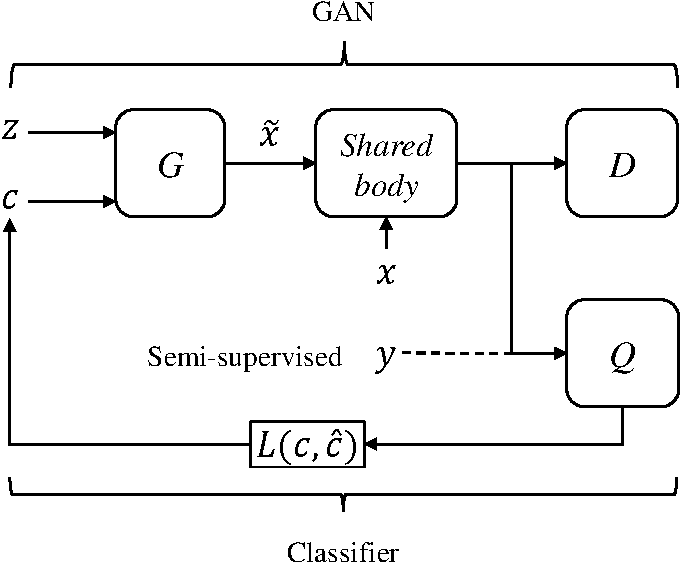
\includegraphics[width=\onef\textwidth]{Img/arch-cinfogan.pdf} 
  \bicaption[C-InfoGAN模型结构示意]
  {C-InfoGAN模型结构。无监督情况下,生成数据$\tilde{\bd{x}}$和真实数据$\bd{x}$参与训练,通过和$D$共享部分结构,$Q$网络可以将GAN模型学习到的特征加以利用,实现分类任务;在半监督情况下,一部分真实标签$y$会直接被$Q$网络利用,以得到更好的效果。模型通过优化$Q$网络的输出$\hat{c}$和隐变量$c$构成的损失函数$L(c,\hat{c})$来增加$Q$的分类准确率。}
  {The architecture of C-InfoGAN. In unsupervised case, the generated data $\tilde{\bd{x}}$ and the real data $\bd{x}$ are used for training. By sharing the body with $D$, $Q$ is able to using features learned by GAN framework to perform classification. In semi-supervised case, labels $y$ is directly fed into $Q$ to get better performance. We optimize the loss function $L(c, \hat{c})$ of latent code $c$ and the output $\hat{c}$ of $Q$ to improve its accuracy.}
  \label{fig:c-infogan}
\end{figure}

使用InfoGAN做分类并不是一个新的想法,\citet{zhang2018cramer}基于InfoGAN提出了一种无监督分类方法。他们生成对抗网络训练的同时,训练一个Parital Inverse Filter (PIF),它接受一个样本作为输入,输出一个和隐变量同维度的向量。之所以叫做PIF,是因为它可以看作生成器$G$的逆映射,将数据映射到隐空间,但又不是完全还原输出噪声,它只输出噪声中的隐变量部分。在训练过程中,他们将PIF的输出与隐变量作均方误差,使得PIF的输出和隐变量的取值尽可能接近。事实上,这个PIF和InfoGAN中的辅助网络具有类似的作用,都是和输入噪声中的隐变量发生联系,而实践发现,使用$Q$网络做分类已经具有可观的效果,而且对计算量的增加较小,模型结构也相对简单。

算法~\ref{alg:cig}给出了C-InfoGAN的训练步骤,其中$\theta_g,~\theta_d,~\theta_q$分别是$G, ~D$和$Q$的网络参数。
\begin{algorithm}[htbp]
  \small
  \caption{Training procedure for C-InfoGAN}
  \label{alg:cig}
  \begin{algorithmic}[1]
    \For{numbers of training iterations}
      \State Sample a batch of $\bd{x} \sim p_{\text{data}}(x)$ of size $m$.
      \State Sample a batch of noise $\bd{z}\sim p_z, ~\bd{c}\sim p_c$ of size
      $m$.
      \State Update the discriminator by ascending its stochastic gradient:
      \[
        \nabla_{\theta_d} \left[ 
          \frac{1}{m} \sum_{i=1}^m \Big( 
            \log D\left(\bd{x}_i\right) + 
            \log\left( 1 - D\left( G(\bd{z}_i, \bd{c}_i) \right) \right)
          \Big)
        \right].
      \]
      \State Update $G$ and $Q$ by descending along its stochastic gradient:
      \[
        \nabla_{\theta_g,\theta_q} \left[ 
          \frac{1}{m} \sum_{\tilde{\bd{x}}} \Big(
            \log(1 - D(G(\bd{z},\bd{c}))) -
            p(\bd{c})\log Q(G(\bd{z}, \bd{c}))
          \Big)
        \right].
      \]
    \EndFor
  \end{algorithmic}
\end{algorithm}


\subsection{半监督分类方法}
%无监督的InfoGAN虽然已经取得非常好的生成效果,但是分类准确率并不是很高。一个自然的想法是通过添加少量标签信息能否使得生成效果更好,分类更准确?答案是肯定的。特别的,
当拥有少量标签信息时,C-InfoGAN可以利用这些标签进一步提升分类准确率和生成效果。同时将隐变量$c$直接绑定到真实的标签,实现精准调控。
%我们可以通过添加少量的标签信息,
%指导隐变量$c$更好地绑定到类别特征,实现精确地调控。
%另外,精确绑定到类别特征的隐变量$c$可以作为直接作为数据的真实标签使用。也就是说,当我们设定$c=1$的时候,生成器就会生成真实类别为`1'的数据。此时,$\argmax_c Q(c|\bd{x})$即可作为分类器的预测值。
针对拥有少量标注信息的情况,\citet{spurr2017guiding}提出半监督的InfoGAN模型,称为ss-InfoGAN。图~\ref{fig:arch-ssinfogan}给出了其模型结构\footnote{ss-InfoGAN模型结构图摘自\citet{spurr2017guiding}。},ss-InfoGAN将隐变量$c$进一步分解为无监督部分$c_{us}$,负责捕捉大量无标注数据的潜在特征;和有监督部分$c_{ss}$,负责捕捉已有标签$y$。同时他们设置了两组隐变量对应的先验分布$P_{c_{us}}$和$P_{c_{ss}}$,以及对应的辅助网络$Q_{us}$和$Q_{ss}$,使用隐变量$c_{ss}$和辅助网络$Q_{ss}$专门处理那部分有标注信息。
\begin{figure}[htbp]
  \centering
  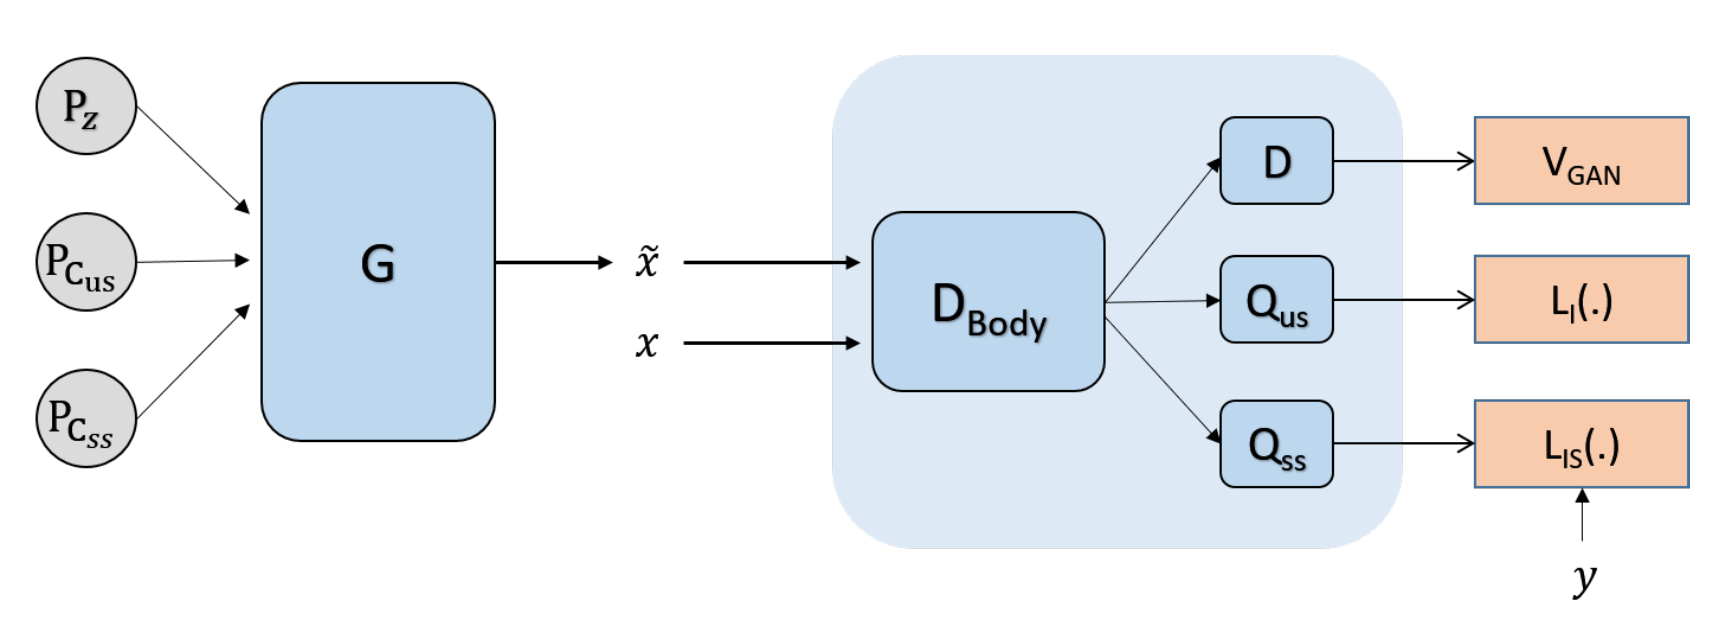
\includegraphics[width=\onef\textwidth]{Img/arch-ssinfogan.png}
  \bicaption{ss-InfoGAN结构示意}{The architecture of ss-InfoGAN}
  \label{fig:arch-ssinfogan}
\end{figure}
本文直接将标签信息加入$Q$网络,先用真实数据和标签训练,接着用生成数据和虚假标签(即隐变量$c$)来训练,这样做的目的是为了使真实标签的信息流入隐变量$c$中,或者可以说是用真实标签指导$c$绑定到正确的类别特征。经过实践发现,简单地使用上述方法也能达到同样的效果,而且模型更为简单。使用和\ref{sec:ss-catgan}节中类似的方法,可以得到半监督C-InfoGAN的目标函数如下:
\begin{equation}\label{eq:ss-cinfogan-obj}
  \begin{split}
  \min_{G,Q}\max_D~ &V_{\text{ss-CIG}}(G,D,Q,\lambda_1,\lambda_2,\lambda_3) = 
  V_{\text{CIG}}(G,D,Q,\lambda_1,\lambda_2) + \\
  &\lambda_3 \E_{(\bd{x}, \bd{y}) \in \Set{L}}
  \left[ \CE[\bd{y}, Q(y|\bd{x})] \right].
  \end{split}
\end{equation}
其中$\lambda_3$为正则化系数,模型结构参见图~\ref{fig:c-infogan}。

算法~\ref{alg:ss-cig}给出了半监督版本的C-InfoGAN的训练步骤,其中$\theta_g, ~\theta_d, ~\theta_g$分别为$G, ~D$和$Q$的网络参数。可以看到,第\ref{ln:bid}行直接将有标签数据放入$Q$网络中训练,通过$Q$网络让标签信息流入虚假标签。在这种情况下,训练稳定之后绑定到类别的隐变量能够和真实标签一一对应(参见~\ref{sec:results}节)。在半监督学习中,如何充分利用有标签数据是一个很重要的问题。在算法~\ref{alg:ss-cig}中,
%做成功概率为$p$的Bernoulli试验。用随机变量$X$表示试验结果,
采用投掷硬币的方式决定如何采样。投掷一枚不公平硬币,正面向上的概率为$p$。设随机变量$X$表示投掷一次该硬币产生的结果,如正面向上,则$X=1$,反之$X=0$,
显然$X\sim\text{Bern}(p)$。
每一次采样前,投掷一次硬币,如果正面向上,则从有标签的数据中采样,否则从无标签数据采样。随着迭代次数的增加,逐渐减小成功概率$p$至某个确定的值。这样做的好处是当$p$减小到最小值之后,虽然由无标签数据占据主导,但还是会偶尔出现一两个有标签的数据批次参与训练,给予无监督训练一定的指导。
\begin{algorithm}[htbp]
  \small
  \caption{Training procedure for semi-supervised C-InfoGAN}
  \label{alg:ss-cig}
  \begin{algorithmic}[1]
    \For{numbers of training iterations}
      \State Sample \texttt{flag} from $\text{Bern}(p)$.
      \Comment{Toss a coin to decide whether to use labels}
      \If{\texttt{flag} is 1}
        \State Sample a batch of labeled samples 
               $(\bd{x}, y) \sim p_{\text{data}}(x,y)$ of size $m$.
      \Else
        \State Sample a batch of unlabeled samples $\bd{x} \sim p_{\text{data}}(x)$ of
        size $m$.
      \EndIf
      \State Sample a batch of noise $\bd{z}\sim p_z, ~\bd{c}\sim p_c$ of size
      $m$.
      \State Update the discriminator by ascending its stochastic gradient:
      \[
        \nabla_{\theta_d} \left[ 
          \frac{1}{m} \sum_{i=1}^m \Big( 
            \log D\left(\bd{x}_i\right) + 
            \log\left( 1 - D\left( G(\bd{z}_i, \bd{c}_i) \right) \right)
          \Big)
        \right].
      \]
      \If{\texttt{flag} is 1}
        \State Update $Q$ by ascending its stochastic gradient: \label{ln:bid}
        \Comment{Bind real labels to fake}
        \[
          \nabla_{\theta_q} \left[ 
            \frac{1}{m} \sum_{(\bd{x}, y)} p(y|\bd{x}) \log Q(\bf{x}) 
          \right].
        \]
      \EndIf
      \State Update $G$ and $Q$ by descending along its stochastic gradient:
      \[
        \nabla_{\theta_g,\theta_q} \left[ 
          \frac{1}{m} \sum_{\tilde{\bd{x}}} \Big(
            \log(1 - D(G(\bd{z},\bd{c}))) -
            p(\bd{c})\log Q(G(\bd{z}, \bd{c}))
          \Big)
        \right]. \label{ln:test}
      \]
      \State $p \gets \max(0.01, \text{Annealing}(p, iterations))$ 
      \Comment{Gradually anneals $p$ to 0.01}
    \EndFor
    %\Procedure{Euclid}{$a,b$}\Comment{The g.c.d. of a and b}
    %\State $r\gets a\bmod b$
    %\While{$r\not=0$}\Comment{We have the answer if r is 0}
    %\State $a\gets b$
    %\State $b\gets r$
    %\State $r\gets a\bmod b$
    %\EndWhile\label{euclidendwhile}
    %\State \textbf{return} $b$\Comment{The gcd is b}
    %\EndProcedure
  \end{algorithmic}
\end{algorithm}

%----------------------------------------------------------------------
\section{InfoCatGAN}\label{sec:icg}
生成对抗网络具有很高的可扩展性,自提出以来应用广泛。\citet{salimans2016improved,odena2016semi}提出使用生成对抗网络模型做半监督分类。在他们的模型中,判别器需要输出$K+1$个类别。考虑一个传统分类模型,给定输入$x$,分类器需要将其分类到$K$个类别中的一个。这样的模型通常接受$x$为输入,输出一个$K$维向量$(\ell_1, \dots, \ell_K)$。通过softmax变换可以将这个向量转化为类别概率$p(y=j|x) = \frac{\exp(\ell_j)}{\sum_{k=1}^K \exp(\ell_k)}$。现考虑使用生成对抗网络做分类,可以通过增加一个类别来对应生成器生成的虚假数据。也就是说,判别器将所有数据分为$K+1$个类别$\Omega = \{\omega_1, \dots, \omega_K, \omega_{K+1}\}$,其中$\omega_{K+1}$对应虚假数据类别。此时,可以用$p(y=\omega_{K+1}|x)$来表示$x$为虚假数据的概率,对应朴素GAN模型中的$1 - D(x)$。对于大量无标签数据,可以通过最大化$\log p(y\in \{\omega_1,\dots,\omega_K\} | x)$来训练分类器。也就是说在给定少量标签的情况下,对于真实数据和虚假数据都有了对应的损失函数
\begin{align}
  L_{\text{ss}} &= -\E_{x,y \sim p_{\text{data}}(x,y)}[\log p(y|x)], \\
  L_{\text{us}} &= -\E_{x\sim p_{\text{data}}(x)}\log [1 - p(y=\omega_{K+1} | x)], \\
  L_{\text{fake}} &= -\E_{x\sim p_g}[\log p(y=\omega_{K+1} | x)],
\end{align}
其中$L_{\text{ss}}, ~L_{\text{us}}, ~L_{\text{fake}}$分别表示针对有标签数据,无标签数据以及虚假数据的损失函数。对于有标签数据,直接利用标签信息优化预测标签和真实标签之间的交叉熵;对于无标签数据,由于标签信息无从得知,所以只能笼统地增加$1-p(y=\omega_{K+1}|x)$来减小被误判的概率;对于虚假数据,都将它判为$\omega_{K+1}$。

\citet{springenberg2015unsupervised}提出的CatGAN模型既可以作无监督分类,也可以做半监督分类。与\citet{salimans2016improved,odena2016semi}类似,CatGAN将判别器扩展为多分类器,令其输出$K$个类别的概率。不同的是,CatGAN重新设计了基于条件熵的损失函数(参见~\ref{sec:catgan})。本节在CatGAN的基础上,添加互信息约束,提出InfoCatGAN模型。该模型同样支持无监督和半监督分类,但是其在生成图片的质量上优于CatGAN。

%\textcolor{red}{improved gan triple gan enhanced triplegan}


\subsection{无监督分类方法}\label{sec:icg-us}
在训练概率分类模型的过程中,通过优化条件熵可以将分类边界调整到更自然的位置(数据分散区域)\cite{grandvalet2005semi},因此CatGAN使用条件熵作为判别器判断真假数据的依据。但是,使用熵作为目标函数的一个缺点是没有类别指向性。考虑一个离散随机变量$Y$表示给定输入$\mathbf{x}$对应的标签,$Y$可能的取值为$\Supp(Y) = \Omega =\{\omega_1, \dots, \omega_K\}$。如果模型仅仅最小化$H(Y|\mathbf{x})$,那么它无法预测$\mathbf{x}$的具体类别。因为任何一个单峰分布都可以使得条件熵达到最小,即$K$个类别中任意一个都可以使$p(y|\mathbf{x})$呈单峰分布,见图~\ref{fig:ent}。
\begin{figure}[htbp]
  \centering
  \begin{subfigure}[b]{\trif\textwidth}
    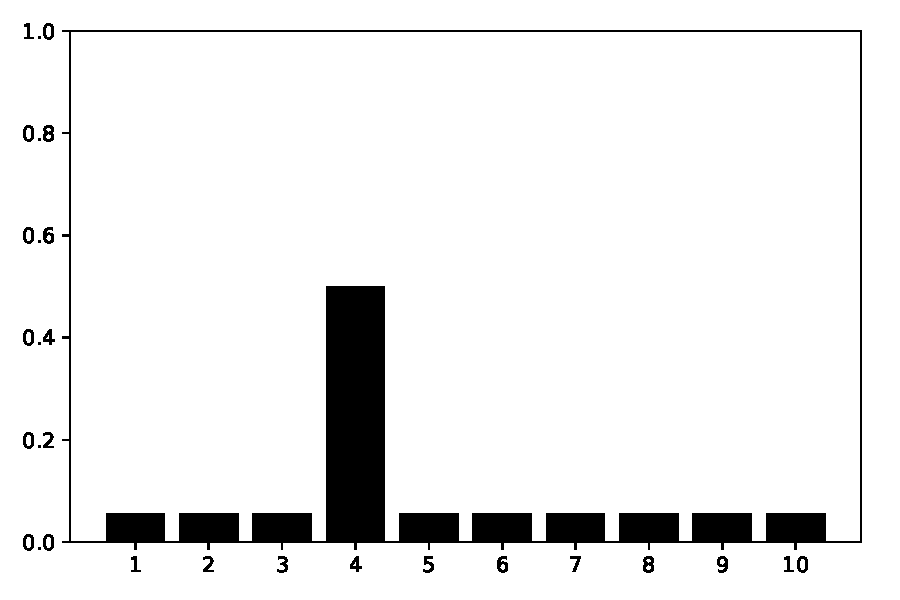
\includegraphics[width=\textwidth]{Img/enta.pdf}
    \caption{$H = 2.58$, predict $y=4$}
  \end{subfigure}
  \begin{subfigure}[b]{\trif\textwidth}
    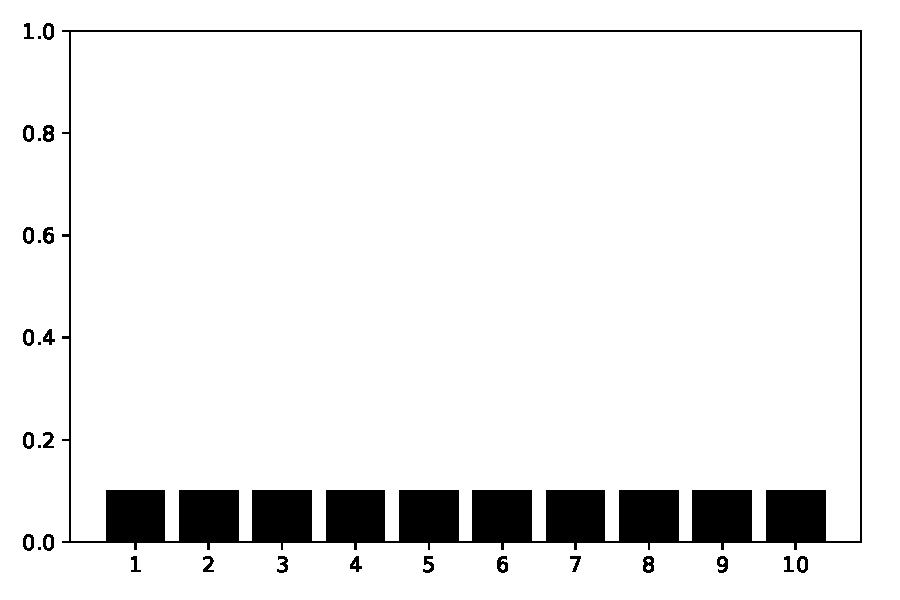
\includegraphics[width=\textwidth]{Img/entb.pdf}
    \caption{$H = 3.32$}
  \end{subfigure}
  \begin{subfigure}[b]{\trif\textwidth}
    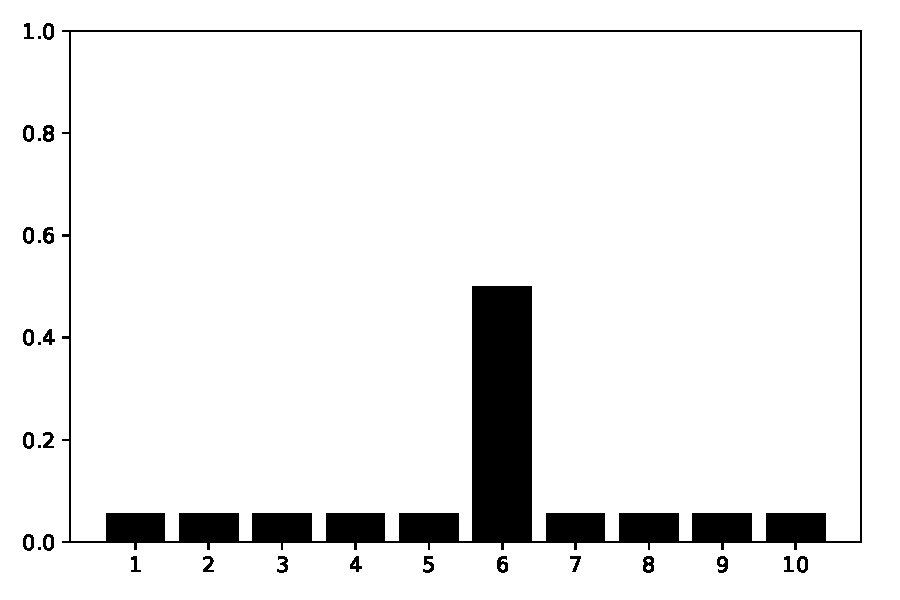
\includegraphics[width=\textwidth]{Img/entc.pdf}
    \caption{$H = 2.58$, predict $y=6$}
  \end{subfigure}
  \bicaption{不同分布的熵}{Entropy of different distributions}
  \label{fig:ent}
\end{figure}
对于分类器而言,希望对于给定输入$\mathbf{x}$,有且仅有一个$k \in [K]$,使得$p(y=\omega_k|\mathbf{x})$最大,而对于任意$k' \neq k, ~p(y=\omega_{k'}|\mathbf{x})$均很小。然而问题在于训练数据集没有标注,每个数据样本对应的标签无从获得。

对于上述问题本文从InfoGAN中获得启发,提出InfoCatGAN模型。InfoGAN将输入噪声划分为$\mathbf{z}$和$\mathbf{c}$,实际上是对隐空间的结构进行了人为划分。一部分提供模型的容量,使得模型具有足够的自由度去学习数据的细节(高度耦合的特征);一部分提供隐变量,用于在学习过程中绑定到数据的显著特征(如:MNIST中的数字类别、笔画粗细、角度)。模型的核心思想如下:通过在隐空间构造一维隐变量$c$,在训练过程中将生成数据的类别标签与之绑定,使得可以通过$c$来控制生成数据的类别。
CatGAN对GAN的扩展主要在于改变了判别器的输出结构:为所有真实数据分配一个类别标签而对于虚假数据则保持一个不确定的状态。类似的,生成器应该致力于生成某个具体类别的数据而不是仅仅生成足够逼真的图片。因此,构造的隐变量实际上充当了虚假图片的标签,它在训练过程中约束着生成器生成指定类别的图片。

\begin{figure}[htbp]
  \centering
  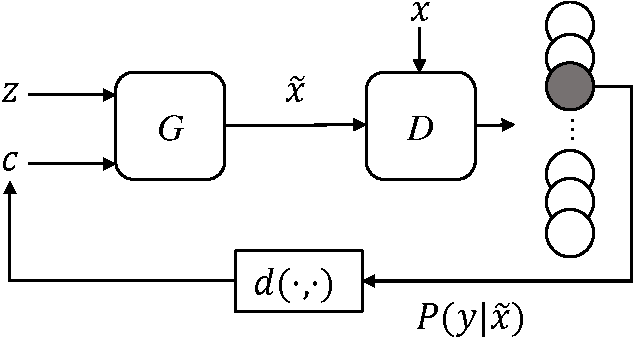
\includegraphics[width=\onef\textwidth]{Img/icg-arch.pdf} 
  \bicaption[InfoCatGAN结构示意]
  {InfoCatGAN模型结构。图中$D$的输出为$P(y|\cdot)$。在训练生成器的时候,将判别器的输出$P(y|\tilde{\mathbf{x}})$和隐变量$c$通过某种度量$d(\cdot, \cdot)$建立联系使得条件概率的峰值与$c$的取值对应。}
  {The architecture of InfoCatGAN. The discriminator outputs $P(y|\cdot)$. When training generator, we add a regularizer $d(\cdot,\cdot)$ between the ouput of discriminator and the latent code $c$ to match the peak of $P(y|\tilde{\mathbf{x}})$ with $c$.}
  \label{fig:icg-arch}
\end{figure}

下面给出InfoCatGAN的损失函数:设$\mathbf{x} \in \mathcal{X}$为一个真实数据样本,$\tilde{\mathbf{x}} = G(\mathbf{z}, c)$为一个生成数据,其中$z\sim p_z$为噪声,$c\sim p_c$为隐变量。为了简单起见,这里只考虑$c$为一维离散随机变量,$p_c$为离散均匀分布。生成器$G = G(\mathbf{z}, c; ~\theta_G)$和判别器$D = D(\mathbf{x}; ~\theta_D)$均为可微深度神经网络,其中$\theta_G, ~\theta_D$分别为生成器和判别器的参数\footnote{参数通常省略。}。通过在$D$网络的最后一层做softmax变换,可以直接将$D(x)$作为条件概率$p(y|x)$的估计。注意到\eqref{eq:catgan-obj}式可以重写为:
\begin{align}
  L_D^{\text{cat}} &= -I(X;Y)-
         \E_{\tilde{\mathbf{x}} \sim p_g}[H(p(y|\tilde{\mathbf{x}}))], \label{eq:lcatd} \\
  L_G^{\text{cat}} &= -I(\tilde{X}; Y), \label{eq:lcatg}
\end{align}
%%NOTE%%
% May have interaction with information bottleneck!
其中$X \sim p_{\text{data}}, ~\tilde{X} \sim p_g$分别表示真实数据和虚假数据对应的随机变量,$Y$表示未知标签对应的随机变量。从\eqref{eq:lcatd}、\eqref{eq:lcatg}式可以看出,CatGAN在优化数据与标签之间的互信息。互信息是常用的变量间相关性的衡量标准,所以本文用它作为生成器损失函数的正则项,由此得到InfoCatGAN的损失函数如下:
\begin{equation}
\label{eq:infocatgan}
\begin{split}
  L_D &= L_D^{\text{cat}}, \\ 
  L_G &= L_G^{\text{cat}} - \lambda_1 I(c; \tilde{\mathbf{x}}),
\end{split}
\end{equation}
其中$\lambda_1$为正则系数,可知当$\lambda_1 = 0$时,InfoCatGAN退化为CatGAN,模型结构见图~\ref{fig:icg-arch}。参考\eqref{eq:infogan-obj}式,$I(c; \tilde{\mathbf{x}})$可以放缩为$\E_{p(\mathbf{c},\tilde{\mathbf{x}})}[\log p(c|\tilde{\mathbf{x}})]$,在实现中通常使用交叉熵
\begin{equation}
  CE[\mathbf{c}, p(c|\tilde{\mathbf{x}})] = -\sum_{i=1}^K c_i \log p(c=c_i | \tilde{\mathbf{x}})
\end{equation}
来优化此项,这里的$\mathbf{c} \in \reals^K$是隐变量$c$经过one-hot编码之后的向量,$p(c|\tilde{\mathbf{x}})$可以用$D(\tilde{\mathbf{x}})$来近似。

算法~\ref{alg:icg}给出了InfoCatGAN的训练步骤,其中$\theta_g,~\theta_d$分别为$G, ~D$的网络参数。第\ref{ln:catd}、\ref{ln:catg}行的更新公式可以参考\eqref{eq:infocatgan}式和\eqref{eq:catgan-obj}式。从第~\ref{ln:catg}行可以看出,算法在训练过程中将隐变量有意识地和虚假图片的类别绑定,这样做的效果是训练稳定后,可以通过隐变量控制生成图片的类别。注意到第\ref{ln:catd}、\ref{ln:catg}行的最后一项分别对应着\eqref{eq:catgan-obj}中的$H_{\Set{X}}(p(y))$和$H_{G}(p(y))$,\citet{springenberg2015unsupervised}指出边缘分布的熵的估计方法应当视情况而定。原本$H_{\Set{X}}$应当针对整个训练数据集来计算边缘分布,然后在计算熵;而$H_G$也不能单单只用一个批次的虚假样本计算,应当生成远大于批处理大小的虚假样本来计算边缘分布,再计算熵。但是在批处理大小$m$远大于类别总数$K$(比如$K=10, ~m=100$)的时候,算法~\ref{alg:icg}中对于边缘分布的熵的估计是合理的\footnote{本文在实验中也采用了校正后的边缘分布的熵的估计方法,发现这对实验结果影响并不大。}。
\begin{algorithm}[htbp]
  \small
  \caption{Training procedure for InfoCatGAN}
  \label{alg:icg}
  \begin{algorithmic}[1]
    \For{numbers of training iterations}
      \State Sample a batch of $\bd{x} \sim p_{\text{data}}(x)$ of size $m$.
      \State Sample a batch of noise $\bd{z}\sim p_z, ~\bd{c}\sim p_c$ of size
      $m$.
      \State Update the discriminator by ascending its stochastic gradient:
      \label{ln:catd}
      \[
        \nabla_{\theta_d} \left[ 
          \frac{1}{m} \sum_{i=1}^m \Big( 
            - H(D(\bd{x}_i)) + H(D(G(\bd{z}_i, \bd{c}_i)))
          \Big) + H\left( \frac{1}{m}\sum_{i=1}^m D(\bd{x}_i) \right)
        \right].
      \]
      \State Update $G$ and $D$ by descending along its stochastic gradient:
      \label{ln:catg}
      \[
        \nabla_{\theta_g,\theta_d} \left[ 
          \frac{1}{m} \sum_{\tilde{\bd{x}} = G(\bd{z},\bd{c})} \Big(
            H(D(\tilde{\bd{x}})) - p(\bd{c})\log D(\tilde{\bd{x}})
          \Big)
          - H \left( 
            \frac{1}{m}\sum_{i=1}^m D(G(\bd{z}_i, \bd{c}_i))
          \right)
        \right].
      \]
    \EndFor
  \end{algorithmic}
\end{algorithm}


\subsection{半监督分类方法}\label{sec:ss-infocatgan}
%%%------> \textcolor{red}{目标写两页}
作为CatGAN的扩展,InfoCatGAN能够很自然地适用于半监督的情况。假设$\Set{L} = \{\mathbf{x}_i, y_i\}_{i=1}^m$为$m$个有标签的样本,$\mathbf{y}_i \in \reals^K$表示标签$y_i$经过one-hot编码之后的向量:即如果$\mathbf{x}_i$的标签是$\omega_k$,则$\mathbf{y}_{ik}=1$且对于所有的$j\neq k,~\mathbf{y}_{ij} = 0$。对于有标签的样本,$D(\mathbf{x})$的分布信息可以明确获得,所以可以通过计算$\mathbf{y}$和$p(y|\mathbf{x})$之间的交叉熵:
\begin{equation}
  \label{eq:celoss}
  \CE[\mathbf{y}, p(y|\mathbf{x})] = -\sum_{i=1}^K y_i \log p(y=y_i | \mathbf{x})
\end{equation}
来辅助判别器做出更精确的判断。半监督版本的InfoCatGAN损失函数如下:
\begin{equation}
  \label{eq:ss-infocatgan-obj}
  L_D^L = L_D + \lambda_2 \E_{(\mathbf{x}, \mathbf{y}) \in \Set{L}}\left[ CE[\mathbf{y}, p(y|\mathbf{x})] \right],
\end{equation}
其中$\lambda_2$为正则系数而生成器的损失函数同\eqref{eq:infocatgan}式:$L_G^L = L_G$.

\begin{algorithm}[htbp]
  \small
  \caption{Training procedure for semi-supervised InfoCatGAN}
  \label{alg:ss-icg}
  \begin{algorithmic}[1]
    \For{numbers of training iterations}
      \State Sample \texttt{flag} from Bern($p$).
      \If{\texttt{flag} is 1}
        \State Sample a batch of labeled samples 
        $(\bd{x}, y) \sim p_{\text{data}}(x,y)$ of size $m$.
      \Else
        \State Sample a batch of unlabeled samples 
        $\bd{x} \sim p_{\text{data}}(x)$ of size $m$.
      \EndIf
      \State Sample a batch of noise $\bd{z}\sim p_z, ~\bd{c}\sim p_c$ of size
      $m$.
      \State Update the discriminator by ascending its stochastic gradient:
      \label{ln:catdss}
      \[
        \nabla_{\theta_d} \left[ 
          \frac{1}{m} \sum_{i=1}^m \Big( 
            - H(D(\bd{x}_i)) + H(D(G(\bd{z}_i, \bd{c}_i)))
          \Big) + H\left( \frac{1}{m}\sum_{i=1}^m D(\bd{x}_i) \right)
        \right].
      \]
      \If{\texttt{flag} is 1}
        \State Update $D$ by ascending its stochastic gradient:
        \label{ln:bidd}
        \[
          \nabla_{\theta_d} \left[ 
            \frac{1}{m} \sum_{(\bd{x}, y)} p(y|\bd{x}) \log D(\bf{x}) 
          \right].
        \]
      \EndIf
      \State Update $G$ and $D$ by descending along its stochastic gradient:
      \label{ln:catgss}
      \[
        \nabla_{\theta_g,\theta_d} \left[ 
          \frac{1}{m} \sum_{\tilde{\bd{x}} = G(\bd{z},\bd{c})} \Big(
            H(D(\tilde{\bd{x}})) - p(\bd{c})\log D(\tilde{\bd{x}})
          \Big)
          - H \left( 
            \frac{1}{m}\sum_{i=1}^m D(G(\bd{z}_i, \bd{c}_i))
          \right)
        \right].
      \]
      \State $p \gets \max(0.01, \text{Annealing}(p, iterations))$ 
    \EndFor
  \end{algorithmic}
\end{algorithm}
算法~\ref{alg:ss-icg}给出了半监督版本的InfoCatGAN的训练步骤,其中$\theta_q,~\theta_d$分别为$G,~D$的网络参数。从第\ref{ln:bidd}行可以看出,如果当前批次是有标签的数据,则直接最小化真实标签和预测概率之间的交叉熵。这样做的目的是通过判别器$D$将真实标签信息流入虚假标签,即隐变量中。训练稳定之后,虚假标签和真实标签会一一对应(参见~\ref{sec:results}节)。在半监督版本的训练中,首先将数据集分为有标签部分和无标签部分,这里同样采用投掷硬币的方式,决定从哪个数据集采样。

\section{本章小结}
本章首先介绍了生成对抗网络的可扩展性:可以添加条件信息学习条件分布;可以增加逆向网络,通过数据空间推断隐空间;可以加入少量标签与半监督学习结合。接着介绍了本文提出的两个模型:C-InfoGAN和InfoCatGAN,这两个模型都可以做到无监督和半监督的分类,并且都利用了互信息约束。第一节详细阐述了无监督和半监督C-InfoGAN的模型结构及理论,并给出了具体的训练算法。第二节详细阐述了无监督和半监督InfoCatGAN的模型结构及理论,并给出了相应的训练算法。具体的实现细节和实验结果将在第\ref{chap:experiments}章给出。

%\chapter{模型评估}\label{chap:experiments}
本章将在MNIST\citep{lecun1989backpropagation}和FashionMNIST\citep{xiao2017/online}数据集上评估模型。MNIST是深度学习广泛使用的评价模型的基础数据集,它包含60000个训练样本,10000个测试样本,每个样本均为$28\times 28$的灰度手写数字图片。FashionMNIST具有和MNIST相同的数据结构,同样是60000个训练样本和10000个测试样本,每个样本均为$28\times 28$灰度图片,也具有10个类别。然而相比于MNIST,FashionMNIST的图片构成更复杂,因此对模型具有更大的挑战。

在所有实验中,本文主要考察两个指标:分类准确率和图片生成质量。对于分类准确率,计算模型预测值并不像一般分类器那样直接。隐变量虽然可以学习到数据类别的特征,但是其取值并不一定和真实标签正确对应(例如$c=1$对应生成真实标签为$\omega_2$的数据)。因此不能直接使用隐变量的取值作为模型的预测值,必须将隐变量的取值与真实标签之间做一个映射。

对于这个问题,本文采取与\citet{springenberg2015unsupervised}类似的做法。首先在测试集上选取$t$个测试样本$\Set{X}_t = \{\mathbf{x}_i, y_i\}_{i=1}^t$,计算模型在这批数据上的预测概率矩阵
\[
  \mathbf{P} = 
\begin{bmatrix}
  p_{11} & p_{12} & \cdots & p_{1k} \\
  p_{21} & p_{22} & \cdots & p_{2k} \\
  \vdots & \vdots & \ddots & \vdots \\
  p_{t1} & p_{t2} & \cdots & p_{tk}
\end{bmatrix},
\]
其中$p_{ij} = \Pr(y=\omega_j | \mathbf{x}_i)$表示给定输入样本$\mathbf{x}_i$时,模型预测$y = \omega_j$的概率。然后对每一行选取最大概率的索引作为模型在这批样本上的预测值
\[
  \mathbf{P}^{\star} = (\ell_1, \ell_2, \cdots, \ell_t)^T, \quad \ell_i = \argmax_j p_{ij}.
\]
显然$\ell_i, ~y_i \in \Omega = \{\omega_1, \omega_2, \cdots, \omega_K\}$。定义映射$f: \Omega \to \Omega$,
\[
  f(\ell) = \argmax_y \left( 
    \sum_{\mathbf{x}: \ell(\mathbf{x}) = \ell} \mathbf{1}\left(y(\mathbf{x}), y\right) 
  \right),
\]
其中$\ell(\cdot)$表示模型预测值,$y(\cdot)$表示数据真实标签,$\mathbf{1}(a, b) = 1$当且仅当$a = b$, 否则为零。此时,给定模型预测的虚假标签$\ell$,映射$f$都可以将它映射为真实标签$f(\ell)$。这就完成了虚假标签到真实标签的转换\footnote{在实际应用中,可能会出现某一行的最大值不唯一的情况,此时选择第一个最大值索引作为输出。值得注意的是,这种情况在实验中并不多见。}。简单来说,模型为每一个数据$\mathbf{x}_i$输出对应的概率向量$p(y|\mathbf{x}_i)$,从而分配虚假标签$\ell_i$(概率向量中最大概率对应的索引),然后将预测值和真实标签对比:将虚假标签落入最多的真实标签的取值作为该虚假标签的取值。比如在所有10个被分类为虚假标签$\ell_1$的样本中,有9个真实标签为$\omega_3$,则将虚假标签$\ell_1$映射到真实类别$\omega_3$。

对于图片生成质量,本文采用Fréchet Inception Distance (FID)\citep{heusel2017gans}来进行衡量\footnote{FID一般用于彩色图片,而MNIST数据集是单通道的灰度图片,本文的做法是将单通道复制3份,形成一张RGB彩色图片然后再计算其FID值。},相较于Inception Score\citep{salimans2016improved}只考虑生成数据,FID还利用了真实数据,因此更能反映生成数据和真实数据的差异。FID越小代表生成的图片和真实图片越接近,生成质量越好。

\begin{figure}[htb]
  \centering
  \begin{subfigure}[b]{\trif\textwidth}
    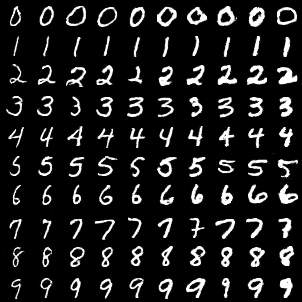
\includegraphics[width=\textwidth]{Img/icg-width.png}
    \caption{$c_2$调控生成数字的粗细}
    \label{ffig:m-icg-witdth}
  \end{subfigure} 
  \begin{subfigure}[b]{\trif\textwidth}
    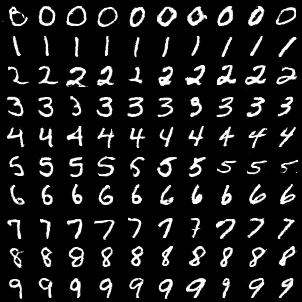
\includegraphics[width=\textwidth]{Img/icg-rotation.png}
    \caption{$c_3$调控生成数字的角度}
    \label{ffig:m-icg-rotation}
  \end{subfigure} 
  \begin{subfigure}[b]{\trif\textwidth}
    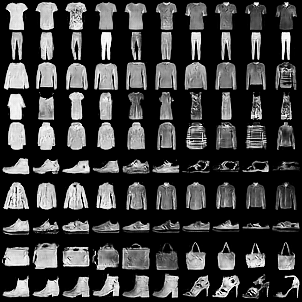
\includegraphics[width=\textwidth]{Img/icg-light.png}
    \caption{$c_2$调控生成图片的亮度}
    \label{ffig:fa-icg-light}
  \end{subfigure} 
  \caption{隐变量对生成图片的调控。图中每一行对应类别隐变量的一个取值,每一列对应其他某个隐变量(固定剩余隐变量)的连续变化。}
  \label{fig:latent-varies}
\end{figure}

\section{实现细节}
在实践中,模型中的所有模块(生成器、判别器、辅助网络等)均被实现为深度神经网络。具体实现可在Github上查看\footnote{实现代码地址:\url{https://github.com/guyueshui/baGAN}}。\textcolor{red}{网络结构在附录中给出。}

\subsection{C-InfoGAN}
对于C-InfoGAN模型,我们的设定和InfoGAN保持大致相同。辅助网络$Q$和判别器$D$共享大部分网络结构,$Q$在判别器的尾部(通常是倒数第二层)分离出一个全连接网络,输出后验概率的估计$Q(\bd{c}|\bd{x})$。因此,C-InfoGAN带来的计算复杂度增加较小。对于离散隐变量$c_i$,在输出之前施加一个softmax激活层,得到的输出代表$Q(c_i|\bd{x})$。对于连续隐变量$c_j$,我们假设其先验分布为高斯分布,然后利用$Q$网络输出它的均值和方差,放到高斯分布中去拟合,计算差值。
由于GAN在训练时容易坍塌,DCGAN\citep{radford2015unsupervised}提出了一种训练稳定的生成对抗网络结构,所以我们采用的网络结构对此有很多参考。关于超参数的选择我们也沿用InfoGAN的设定,对于离散隐变量设置为1;对于连续隐变量,设置为较小的值0.1。

表~\ref{tab:m-cig-netarch}是给出了C-InfoGAN在MNIST上的网络结构,如前所述,判别器$D$和辅助网络$Q$共享大部分网络结构。在MNIST数据集上,噪声空间的构成为一个10维离散隐变量,两个连续隐变量和62维高斯噪声,最终得到的噪声维度为74。对于FashionMNIST,我们在实践中发现使用同样的网络结构也能达到很好的效果。因此本文对于两个数据集采用同样的网络结构。
\begin{table}
  % \renewcommand\arraystretch{0.7} % set row height
  \centering
  \bicaption{C-InfoGAN在MNIST上的网络结构}
  {Architectures of C-InfoGAN used for MNSIT dataset}
  \begin{tabular}{l|l}
    \hline
    \textbf{生成器$G$}               & \textbf{判别器$D$/辅助网络$Q$} \\ \hline
    Input $\in \reals^{74}$          & Input $28\times 28$ Gray image \\ \hline
    fc 1024. bn. relu                & conv 64: k4, s2, p1. lrelu  \\ \hline
    fc $7\times7\times128$. bn. relu & conv 128: k4, s2, p1. bn. lrelu \\ \hline
    upconv 64: k4, s2, p1. bn. relu  & fc 1024. bn. lrelu \\ \hline
    upconv 1: k4, s2, p1. tanh       & fc 1. sigmoid. output for $D$, \\
    ~                                & fc 128. bn. lrelu. fc. output for $Q$ \\
    \hline
  \end{tabular}
  \label{tab:m-cig-netarch}
\end{table}

\subsection{InfoCatGAN}
对于InfoCatGAN,我采用的模型如下。
\begin{table}
  % \renewcommand\arraystretch{0.7} % set row height
  \centering
  \bicaption{InfoCatGAN在MNIST上的网络结构}
  {Architectures of InfoCatGAN used for MNSIT dataset}
  \begin{tabular}{l|l}
    \hline
    \textbf{生成器$G$}               & \textbf{判别器$D$} \\ \hline
    Input $\in \reals^{74}$          & Input $28\times 28$ Gray image \\ \hline
    fc 1024. bn. relu                & conv 64: k4, s2, p1. lrelu  \\ \hline
    fc $7\times7\times128$. bn. relu & conv 128: k4, s2, p1. bn. lrelu \\ \hline
    upconv 64: k4, s2, p1. bn. relu  & fc 1024. bn. lrelu \\ \hline
    upconv 1: k4, s2, p1. tanh       & fc 10. softmax \\
    \hline
  \end{tabular}
  \label{tab:m-icg-netarch}
\end{table}

\section{实验结果}

\subsection{MNIST}\label{sec:icg-ex}

图~\ref{ffig:m-cg}和图~\ref{ffig:m-icg}是在无监督情况下CatGAN和InfoCatGAN的生成效果,可以看到,InfoCatGAN的生成效果明显高于CatGAN,并且每一行基本是一种数字类别,对应隐变量的不同取值。半监督情况下有类似的结果,不同的是在少量标签信息的辅助下,InfoCatGAN可以将隐变量$c$和真实标签正确绑定,$c=1$对应生成数字`1',见图~\ref{ffig:m-ss-icg}。CatGAN生成的图片质量很差,原因在于其目标函数是为了分类而设计的。生成器的作用只是为了判别器能够更加鲁棒,如\ref{sec:icg-us}节所述,从\eqref{eq:catgan-g}式中可以看到,$G$的目标函数只有条件熵,无法针对性地生成图片,从而会降低生成图片的质量。而InfoCatGAN由于增加了隐变量$c$,并在训练过程中有意识地将生成数据的类别与之绑定,所以生成的图片质量较好。

\begin{figure}[htbp]
  \centering
  \begin{subfigure}[b]{\trif\textwidth}
    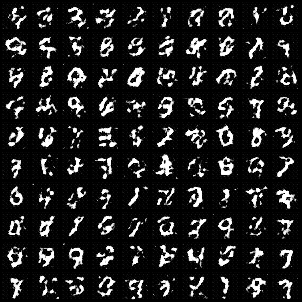
\includegraphics[width=\textwidth]{Img/cg.png}
    \caption{CatGAN}
    \label{ffig:m-cg}
  \end{subfigure}
  \begin{subfigure}[b]{\trif\textwidth}
    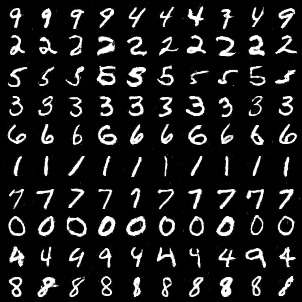
\includegraphics[width=\textwidth]{Img/icg.png}
    \caption{InfoCatGAN}
    \label{ffig:m-icg}
  \end{subfigure}
  \begin{subfigure}[b]{\trif\textwidth}
    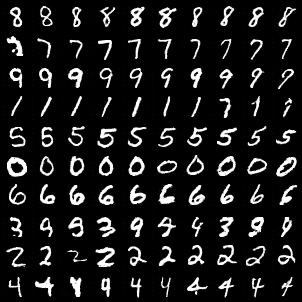
\includegraphics[width=\textwidth]{Img/ig.png}
    \caption{C-InfoGAN}
    \label{ffig:m-ig}
  \end{subfigure}

  \begin{subfigure}[b]{\trif\textwidth}
    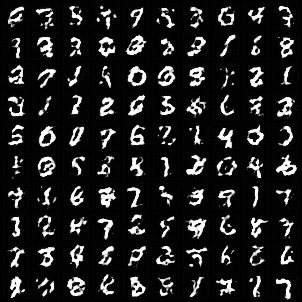
\includegraphics[width=\textwidth]{Img/cg-132labels.png}
    \caption{CatGAN(132 labels)}
    \label{ffig:m-ss-cg}
  \end{subfigure}
  \begin{subfigure}[b]{\trif\textwidth}
    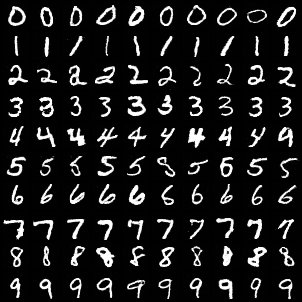
\includegraphics[width=\textwidth]{Img/icg-132labels.png}
    \caption{InfoCatGAN(132 labels)}
    \label{ffig:m-ss-icg}
  \end{subfigure}
  \begin{subfigure}[b]{\trif\textwidth}
    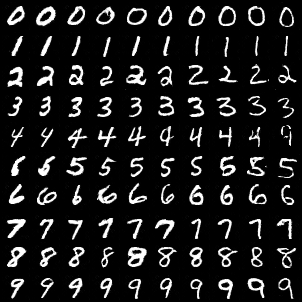
\includegraphics[width=\textwidth]{Img/ig-132labels.png}
    \caption{C-InfoGAN(132 labels)}
    \label{ffig:m-ss-ig}
  \end{subfigure}

  \caption{模型在MNIST上得生成效果。在InfoCatGAN和C-InfoGAN的生成结果中,每一行对应隐变量$c$的一个取值,从0到9。}
  \label{fig:mnist}
\end{figure}

表~\ref{tab:cat}给出了无监督和半监督情况下的分类准确率\footnote{表中有关CatGAN的数据来自与本文复现的结果,与\citet{springenberg2015unsupervised}有所差距。经过多次尝试,我们仍无法完美复现出原文中的结果。}。从表中看出,在无监督的情况下InfoCatGAN的分类准确率相较于CatGAN有所提升,而FID从236.75降低到8.04,图片生成质量有了极大的提升,见图~\ref{ffig:m-icg}。在半监督的情况下,CatGAN的准确率达到了96.05\%,而InfoCatGAN随着正则化系数$\lambda_1$的变化呈现出不同的效果。当系数较小时,分类准确率较高,但生成图片的质量非常差;当系数较大时,生成的图片效果很好,但分类准确率有所降低。通过调节参数$\lambda_1$,可以实现生成效果和分类准确率之间的折中。实验使用的默认值是$\lambda_1 = 1.1$,
当$\lambda_1$减小时,生成图片的质量开始下降,同时分类准确率也会相应增加。值得注意的是,$\lambda_1$越小并不意味着分类准确率越高。当$\lambda_1=0$时,InfoCatGAN退化为CatGAN;而从表~\ref{tab:cat}可以看出,当$\lambda_1=0.02$时,InfoCatGAN的分类准确率高于CatGAN,达到98.15\%。

\begin{table}[htbp]
  \centering
  \caption{MNIST分类准确率对比}
  \label{tab:cat}
  \begin{tabular}{|l|c|c|}
    \hline
    \textbf{模型} & \textbf{准确率(\%)} & \textbf{FID} \\
    \hline
    CatGAN & 64.41 & 236.75  \\ \hline
    InfoCatGAN & 69.04 & 8.04 \\ \hline
    C-InfoGAN & 77.65 & 7.55 \\ \hline
    CatGAN(132 labels) & 96.05 & 127.92 \\ \hline
    InfoCatGAN(132 labels, $\lambda_1 = 0.02$) & \textbf{98.15} & 169.72 \\ \hline
    InfoCatGAN(132 labels, $\lambda_1 = 0.03$) & 80.43 & \textbf{6.59} \\ \hline
    C-InfoGAN(132 labels) & 93.70 & 9.16 \\ \hline
  \end{tabular}
\end{table}

%\textcolor{red}{here begins c-infogan} 
图~\ref{ffig:m-ig}和图~\ref{ffig:m-ss-ig}给出了无监督和半监督情况下C-InfoGAN的生成结果。从图中可以看出无监督情况下,模型已经达到了很好的生成效果,隐变量$c$基本可以控制生成图片的类别,但是仍有部分类别未能精确控制(图~\ref{ffig:m-ig});在半监督情况下,隐变量达到了精确的绑定,每一行对应生成一种类别的数字,而且顺序和真实标签是对应的。另外从图~\ref{fig:latent-varies}可以看出,C-InfoGAN模型不仅可以生成指定类别的图片,并且可以通过额外的隐变量调节图片局部特征,如手写数字的粗细,角度等,这对指定特征的数据补足具有很大意义。

表~\ref{tab:cat}给出了C-InfoGAN的准确率和FID及其与CatGAN模型的性能对比。可以看出,相较于CatGAN模型,C-InfoGAN模型可以获得更高的准确率和生成质量,而且隐变量的绑定效果也更好。而在半监督情况下,C-InfoGAN在保证生成质量的前提下,仍然能够达到93.7\%的分类准确率。这是因为InfoGAN模型使用的是一个辅助网络$Q$来做类别绑定和分类任务,训练过程中并没有判别器做过多约束,所以无论如何调整分类网络或更改分类约束,也不会对生成效果产生很大影响。这使得模型可以进一步利用生成的图片和标签扩充数据集,以达到更进一步的性能提升。

\subsection{FashionMNIST}\label{sec:fashion}

FashionMNIST\citep{xiao2017/online}是一个类似MNIST的数据集,二者拥有同样的结构,图像大小,同样的类别数目。但是相对于MNIST,FashionMNIST拥有更复杂的图像结构,以及更难获得非常高的分类准确率,所以对模型更具有检验性。

表~\ref{tab:fashion}给出了模型在FashionMNIST的数值结果,其中InfoCatGAN的正则系数$\lambda_1 = 0.03$。从表中可以看出,无论是在无监督还是半监督情况下,CatGAN的分类准确率都是比较高的,但从生成效果来看,它却是最差的。在无监督情况下,InfoCatGAN提高了生成图片的质量,但与此同时,牺牲了分类准确率,而C-InfoGAN在一定程度上二者兼顾,不仅生成质量最优,而且具有相对较高的分类准确率,此外其模型复杂度也较低。在半监督情况下,InfoCatGAN在两个方面均体现出优势,分类准确率达到了74.21\%,FID为$16.92$,生成效果见图~\ref{ffig:ss-icg},这说明增加标签信息对模型的增益很大。

\begin{table}[htbp]
  \centering
  \caption{FashionMNIST分类准确率对比}
  \label{tab:fashion}
  \begin{tabular}{|l|c|c|}
    \hline
    \textbf{模型} & \textbf{准确率(\%)} & \textbf{FID} \\
    \hline
    CatGAN & 64.28 & 120.04  \\ \hline
    InfoCatGAN & 57.66 & 26.43 \\ \hline
    C-InfoGAN & 60.50 & 15.97 \\ \hline
    CatGAN(100 labels) & 73.34 & 119.16 \\ \hline
    InfoCatGAN(100 labels) & \textbf{74.21} & 16.92 \\ \hline
    C-InfoGAN(100 labels) & 68.94 & \textbf{15.94} \\ \hline
  \end{tabular}
\end{table}

\begin{figure}[htbp]
  \centering
  \begin{subfigure}[b]{\trif\textwidth}
    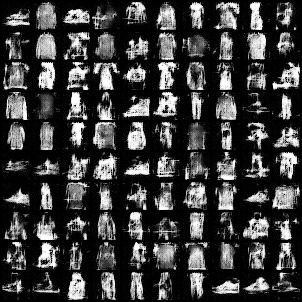
\includegraphics[width=\textwidth]{Img/fa-cg.png}
    \caption{CatGAN}
  \end{subfigure}
  \begin{subfigure}[b]{\trif\textwidth}
    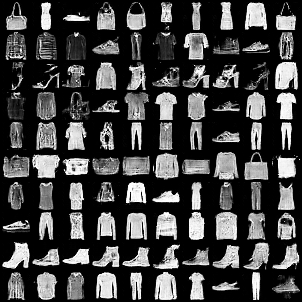
\includegraphics[width=\textwidth]{Img/fa-icg.png}
    \caption{InfoCatGAN}
  \end{subfigure}
  \begin{subfigure}[b]{\trif\textwidth}
    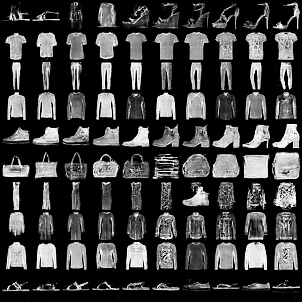
\includegraphics[width=\textwidth]{Img/fa-ig.png}
    \caption{C-InfoGAN}
  \end{subfigure}

  \begin{subfigure}[b]{\trif\textwidth}
    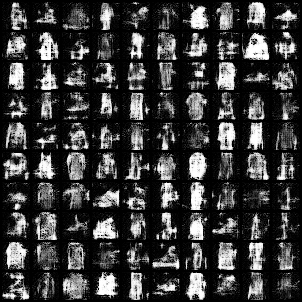
\includegraphics[width=\textwidth]{Img/fa-cg-100labels.png}
    \caption{CatGAN(100 labels)}
  \end{subfigure}
  \begin{subfigure}[b]{\trif\textwidth}
    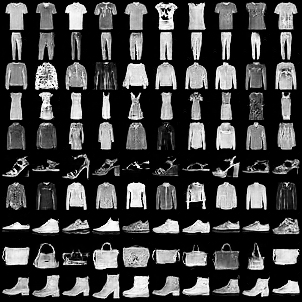
\includegraphics[width=\textwidth]{Img/fa-icg-100labels.png}
    \caption{InfoCatGAN(100 labels)}
    \label{ffig:ss-icg}
  \end{subfigure}
  \begin{subfigure}[b]{\trif\textwidth}
    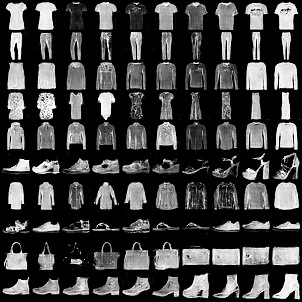
\includegraphics[width=\textwidth]{Img/fa-ig-100labels.png}
    \caption{C-InfoGAN(100 labels)}
    \label{ffig:ss-ig}
  \end{subfigure}

  \caption{模型在FashionMNIST上的生成效果。在InfoCatGAN和C-InfoGAN的生成结果中,每一行对应隐变量$c$的一个取值,从0到9。}
  \label{fig:fashion}
\end{figure}

图~\ref{fig:fashion}中给出了所有模型的生成结果。值得一提的是,加入互信息约束后的半监督版本模型从上往下每一行都对应同一个类别,并且顺序和训练数据的真实标签正确对应(图~\ref{ffig:ss-icg}、\ref{ffig:ss-ig})。这说明了隐变量正确绑定到类别特征,并且可以精准调控生成图片的类别。

\subsection{收敛速度分析}
本文提出的两个模型在原理上都属于正则化生成对抗网络,因此相较于原先的两个模型CatGAN和InfoGAN,增加的计算复杂度很小。由于GAN的训练方式特殊,训练的过程是生成器和判别器的对抗,因此目前没有一个统一的评判收敛性的标准。针对InfoCatGAN和C-InfoGAN两种模型,本文分别用条件熵损失(即判别器输出的概率分布对应的熵)以及互信息损失(实际采用交叉熵估计,详见\ref{sec:cig-us}节)来作为模型收敛的佐证,见图~\ref{fig:convergence}。
\begin{figure}[htbp]
  \centering
  \begin{subfigure}[b]{\twof\textwidth}
    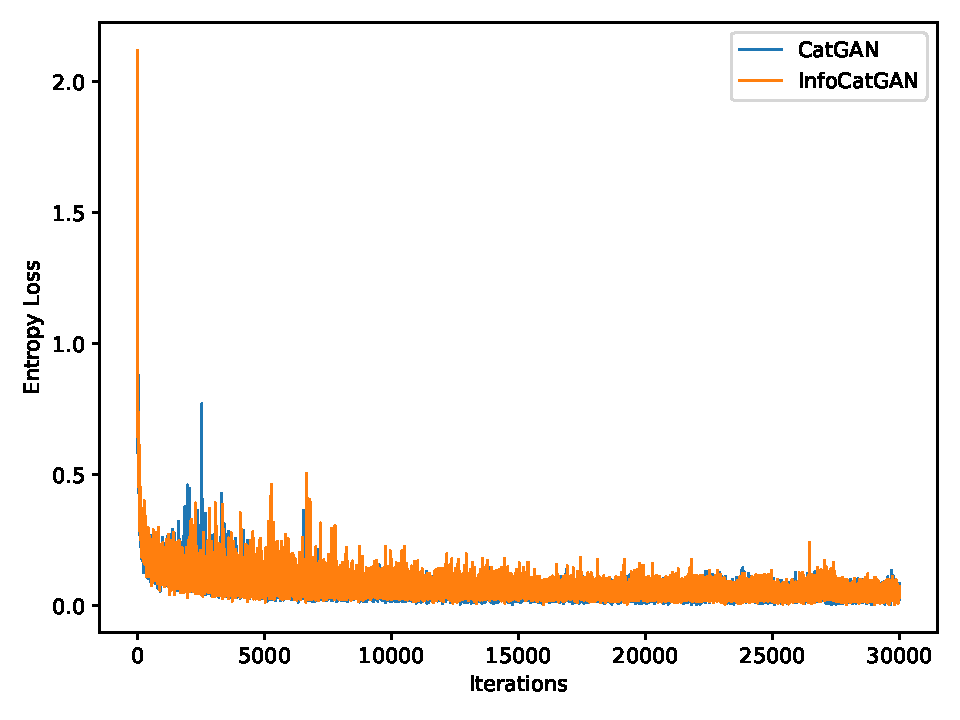
\includegraphics[width=\textwidth]{Img/icg-convergence.pdf}
    \caption{Entropy loss of CatGAN and InfoCatGAN}
    \label{ffig:icg-convergence}
  \end{subfigure}
  \begin{subfigure}[b]{\twof\textwidth}
    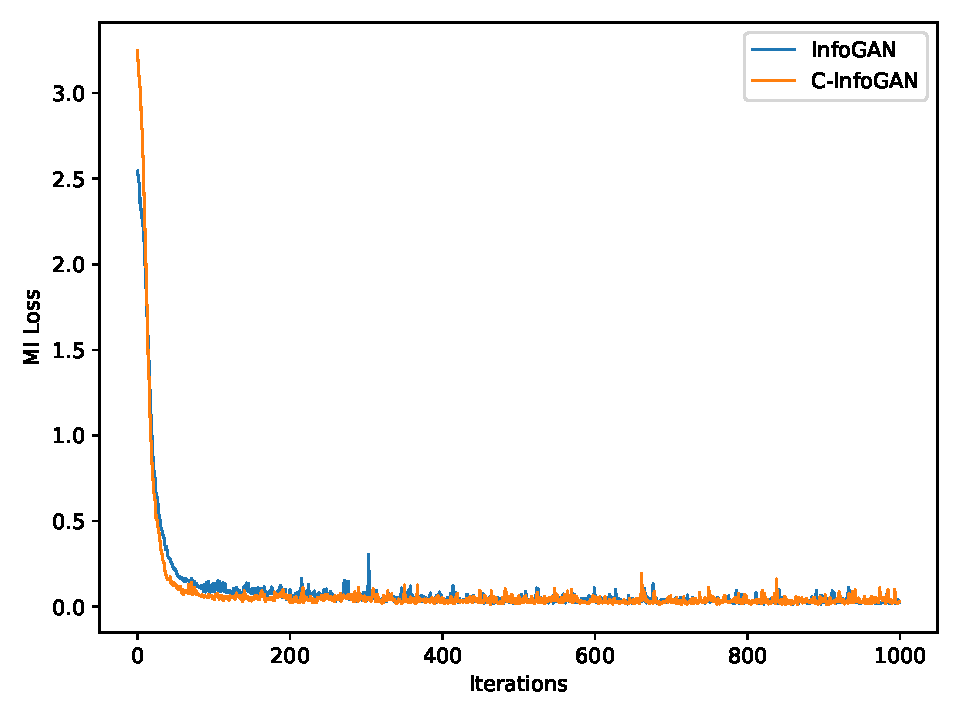
\includegraphics[width=\textwidth]{Img/cig-convergence.pdf}
    \caption{Mutual information loss of InfoGAN and C-InfoGAN}
    \label{ffig:cig-convergence}
  \end{subfigure}
  \bicaption{模型在MNIST上的收敛速度}{Convergence speed on MNIST}
  \label{fig:convergence}
\end{figure}
%\input{Tex/chap_5.tex}
\input{Tex/Chap_Guide}
%---------------------------------------------------------------------------%
% main content
%-
%-> Appendix
%-
% \cleardoublepage%
% \appendix% initialize the environment
% \input{Tex/Appendix}% appendix content
%-
%-> Backmatter: bibliography, glossary, index
%-
\backmatter% initialize the environment
\intotoc*{\cleardoublepage}{\bibname}% add link to toc
\bibliography{Biblio/ref}% bibliography
%---------------------------------------------------------------------------%
%->> Backmatter
%---------------------------------------------------------------------------%
\chapter{作者简历及攻读学位期间发表的学术论文与研究成果}


\section*{作者简历}

胡兵兵,安徽马鞍山人,中国科学院上海微系统与信息技术研究所硕士研究生。

\section*{已发表(或正式接受)的学术论文:}

{
\setlist[enumerate]{}% restore default behavior
\begin{enumerate}[nosep]
    \item \textbf{胡兵兵},唐华,吴幼龙. 基于互信息约束的生成对抗网络分类模型研究,中国科学院大学学报,2020. (尚在评审)
\end{enumerate}
}

% \section*{申请或已获得的专利:}
% 
% (无专利时此项不必列出)
% 
% \section*{参加的研究项目及获奖情况:}
% 
% 可以随意添加新的条目或是结构。

\chapter[致谢]{致\quad 谢}\chaptermark{致\quad 谢}% syntax: \chapter[目录]{标题}\chaptermark{页眉}
\thispagestyle{noheaderstyle}% 如果需要移除当前页的页眉
%\pagestyle{noheaderstyle}% 如果需要移除整章的页眉

不知不觉又过了三个年头,依稀记得三年前我刚来到学校的时候还对硕士生涯充满着未知,不知道这三年又会是什么样的生活。如今回过头来发现,越是学习,越是发现自己不懂的东西很多。犹记得在学习课程时期,经常熬夜到凌晨写作业,做实验的情景;犹记得每天读论文,每周开组会,上台做报告情景;犹记得某些问题弄不懂,抓耳挠腮和同学讨论,请教老师的情景。这些经历都是我宝贵的回忆,以后也会在我前行的道路上给予我动力。

首先我要感谢我的导师吴幼龙。作为一名年轻的教授,他具有严谨的学术态度、专业的知识素养、灵活的思维方式、以及浓烈的科研热情。更难能可贵的是,他平易近人,丝毫没有老师的架子,与学生相处亦师亦友。在求学途中,我的导师总是孜孜不倦、不厌其烦地教导我,经常与我讨论问题到很晚,无论是学习还是生活上,都给予了我莫大的关怀。在完成毕业论文期间,我更是频繁地向他请教问题,讨论实验方案,汇报论文进展,他也非常耐心地为我解答,和我讨论,帮我修改论文。我在此向他表示由衷的感谢!我还要感谢我的同窗们:汪科、马莹莹,以及同组的学弟学妹陈家慧、唐华,他们陪我一起度过了求学的时光,我们经常一起讨论学习和生活上的各种问题。我还要感谢我的学长学姐们:黄曦、高欣、边思梦,他们在我刚来学校的那段时间,给了我很多的帮助,让我能快速地融入学校,适应研究生阶段的学习模式。我也要感谢我的父母,是他们给了我求学的机会,给我提供了生活的基础。此外,我还要感谢我的女朋友尚玉静,她一直默默支持我,鼓励我,陪伴我。都说每个成功男人的背后都有一个伟大的女人,我可能不够成功,她可能不够伟大,但我觉得我们能走到一起这件事就是我最大的成功。

最后,感谢审阅论文的老师们,感谢百忙之中出席答辩的老师们!我在此向所有关心、支持和帮过我的人表示由衷的感谢!

\cleardoublepage[plain]% 让文档总是结束于偶数页,可根据需要设定页眉页脚样式,如 [noheaderstyle]
%---------------------------------------------------------------------------%
% other information
\end{document}
%---------------------------------------------------------------------------%

